\documentclass[11pt, twoside]{article}
\usepackage{multicol}
\usepackage{graphicx} % Required for inserting images
\usepackage[
        inner=30mm,
        outer=20mm, 
        top=25mm,
        bottom=25mm,
        ]{geometry}
\usepackage{lipsum}
\usepackage{polski}
\usepackage{indentfirst}
\usepackage{setspace}
\usepackage{float}
\usepackage{caption}
\usepackage{makeidx}
\usepackage{tocloft}
\usepackage{tocbibind}
\usepackage[backend=biber, sorting=none]{biblatex}
\usepackage{tabularray}
\usepackage{amssymb}
\usepackage{fancyhdr}
\usepackage{amsmath}
\usepackage{pgfplots}
\usepackage{array}
\usepackage{longtable}
\pgfplotsset{compat=1.17}
\usepackage{booktabs}
\usepackage{pdfpages}
\usepackage{listings}
% \usepackage[newfloat]{minted}
\usepackage{tikz}
\usepackage[acronym, toc]{glossaries}
\usetikzlibrary{shapes,arrows, positioning}

\pagestyle{fancy}
\lhead{}
\setlength{\headheight}{1.3em}
\setlength{\parindent}{0.5cm}
\renewcommand\headrulewidth{0pt} % no line between document and header
\fancyhf{}


\renewcommand{\headrulewidth}{1pt}
\renewcommand{\cftsecaftersnum}{.}
\renewcommand{\cftsecleader}{\cftdotfill{\cftdotsep}}
% \let\oldcite\cite
% \renewcommand*\cite[1]{(\oldcite{#1})}
\fancyhead[LE,RO]{\leftmark}
\fancyfoot[RO, LE]{\thepage} % page at left on even and right on odd pages


\addbibresource{src/bibliography/Bibliography.bib}

\def\ThesisPL{Segmentacja lezji stwardnienia rozsianego z wykorzystaniem splotowych
sieci neuronowych}
\def\ThesisEN{Multiple Sclerosis lesion segmentation using convolutional neural networks}

\newcommand{\chapterLink}[1]{\textit{(Rozdział \ref{#1})}}
\newcommand{\en}[1]{\textit{(ang. #1)}}
\newcommand{\la}[1]{\textit{(łac. #1)}}
\newcommand{\picwidth}{0.8}

% \captionsetup[figure]{hangindent=0pt, singlelinecheck=false}
\newcommand{\addImage}[3]{
    \begin{figure}[H]
        \centering
        \includegraphics[width=\picwidth\textwidth]{#2}
        \caption{#3}
        \label{#1}
    \end{figure}
}
\newcommand{\imgRef}[1]{(Rys. \ref{#1})}
\newcommand{\tabRef}[1]{(Tab. \ref{#1})}


\renewcommand{\rmdefault}{qhv}
\setstretch{1.1}

% \newenvironment{code}{\captionsetup{type=listing}}{}
%\SetupFloatingEnvironment{listing}{name=Listing}

\title{Praca Magisterska}
\author{01133546}
\date{October 2023}

\makeindex





\newacronym{ms}{MS}{Stwardnienie rozsiane}
\newacronym{ann}{ANN}{Sztuczne sieci neuronowe}
\newacronym{cnn}{CNN}{Splotowe sieci neuronowe}
\newacronym{mri}{MRI}{Obrazowanie metodą rezonansu magnetycznego}
\newacronym{oun}{OUN}{Ośrodkowy układ nerwowy}
\newacronym{ppv}{PPV}{Precyzja}
\newacronym{npv}{NPV}{Wartość predykcyjna ujemna}
\newacronym{acc}{ACC}{Dokładność}
\newacronym{bacc}{BACC}{Zbalansowana dokładność}
\newacronym{tpr}{TPR}{Czułość}
\newacronym{tnr}{TNR}{Swoistość}
\newacronym{f1}{F1}{Współczynnik Sørensen'a–Dice'a}
\newacronym{mcc}{MCC}{współczynnik korelacji Matthews}
\newacronym{jacc}{JACC}{Indeks Jaccarda}
\newacronym{fnn}{FNN}{Jednokierunkowa sieć neuronowa}
\newacronym{mlp}{MLP}{Perceptron wielowarstwowy}
\newacronym{sgd}{SGD}{Stochastyczna metoda gradientu prostego}
\newacronym{ide}{IDE}{Zintegrowane środowisko programistyczne}
\newacronym{gpu}{GPU}{Procesor graficzny}
\newacronym{cuda}{CUDA}{Compute Unified Device Architecture}
\newacronym{cad}{CAD}{Komputerowo wspomagana diagnostyka medyczna}
\newacronym{bce}{BCE}{Binarna entropia krzyżowa}
\newacronym{fl}{FL}{Funkcja kosztu Focal}
\glsaddall
\makenoidxglossaries

\begin{document}



\begin{titlepage}
\begin{center}
\includegraphics[width = \linewidth]{src/img/util/elka.jpg}\\[5ex]

\fontsize{12}{10}\selectfont
Instytut Radioelektroniki i Technik Multimedialnych\\[6ex]

{
\fontsize{45}{15}\fontfamily{lmtt}\selectfont
Praca dyplomowa magisterska\\[2ex]
}
{
\fontsize{12}{10}\selectfont
\par
na kierunku Inżynieria biomedyczna\\[1ex]
\par
w specjalności Informatyka biomedyczna\\[6ex]
}
{
\Large
\ThesisPL\\[7ex]
}

{
\LARGE
inż. Witold Synowiec\\[1ex]
}
{
Numer albumu 293328\\[5ex]
}
{
\par
promotor\\[1ex]
\par
dr.inż. Robert Kurjata\\[8ex]
}

\vskip 4ex
WARSZAWA, 2023\\

\end{center}
\end{titlepage}
\cleardoublepage
\includepdf[pages={1}]{src/Oswiadczenie_autora_pracy_dyplomowej.pdf}

\cleardoublepage

\begin{spacing}{1.15}

\begin{center}
\section*{\large\ThesisPL} 
\end{center}

%\lipsum[1-3]

Stwardnienie rozsiane (MS) jest jedną z najpowszechniejszych chorób neurodegeneracyjnych, często prowadzącą do niepełnosprawności. Może spowodować utratę lub poważny uszczerbek na wzroku, równowadze, kontroli mięśni, oraz wpływa na codzienną aktywność i pogorszenie zdrowia psychicznego. Jednym ze sposobów diagnozy i kontroli przebiegu MS jest analiza lezji na obrazach MRI. Oznaczanie lezji jest procesem czasochłonnym, wykorzystuje dużą ilość ludzkich zasobów oraz wyniki procesu są różne, w zależności od osoby która je dokonuje. Postuluje się stworzenie narzędzia, potrafiącego w automatyczny sposób oznaczyć lezje. W tym celu przedstawia się splotową sieć neuronową, służącą realizacji opisanego zadania. Powstało wiele publikacji zajmujących się podobną tematyką, jednak często wyniki były niezadowalające. Problemem w uczeniu sieci neuronowych do segmentacji lezji MS jest bardzo duże niezbalansowanie danych. W niniejszym rozwiązaniu proponuje się wykorzystanie ważonych funkcji kosztów do rozwiązania tego problemu. Przedstawione sieci osiągają dobre rezultaty w problematyce segmentacji lezji MS. Do procesu uczenia wykorzystano dane ISBI oraz OFSEP, składające się ze skanów MRI oraz oznaczeń lezji.\\[7ex]


\begin{centering}
\section*{\large\ThesisEN}
\end{centering}

%\lipsum[1-3]

Multiple sclerosis (MS) is one of the most common neurodegenerative illnesses, often resulting in disabilities. It may procure serious harm to vision, balance, muscle control, and also is negatively influencing daily activities and mental health. One of the diagnosis and disease-control method is observation of lesions on MRI scans. Lesion segmentation is a time costly process, it requires a lot of human resources, the result of it may be biased by human views. The tool is proposed, that would be able to automatically perform the lesion segmentation task. For this reason, the convolutional neural network is used, that would handle the task. Great many of publications have been made, often with unsuccessful results. The hardship in training neural networks to perform a lesion segmentation is heavy imbalance of data. In the following solution, the use of a weighted cost function is proposed. Prepared networks do have good results with MS lesion segmentation. The data gathered from ISBI and OFSEP has been used, that contain MRI scans and lesion segmentation ground-truths.
\cleardoublepage

\tableofcontents
\clearpage
%\section*{Wykaz symboli i skrótów}
%\label{sec:intro}
%\addcontentsline{toc}{section}{Wykaz symboli i skrótów}
\glsaddallunused[\acronymtype]
\printnoidxglossary[type=acronym, style=listdotted, title={Wykaz symboli i skrótów},nonumberlist, nogroupskip]




\clearpage

\section{Wprowadzenie}
\label{sec:Introduction}

\par
Niniejsza praca dotyczy dynamicznie rozwijającego się obszaru jakim jest implementacja systemów przetwarzania informacji opartych na sieciach neuronowych w diagnostyce medycznej, tym samym zalicza się do nurtu komputerowo wspomaganej diagnostyki medycznej CAD \en{computer aided diagnosis}. Obserwuje się stały wzrost zainteresowania CAD wraz z pojawiającą się dostępnością nowych technik, a także wraz z usprawnianiem oraz rozszerzaniem istniejących metod akwizycji danych medycznych. W ostatnich latach jedną z najpopularniejszych technik, ze względu na rozwój jednostek obliczeniowych, stały się metody oparte na sztucznych sieciach neuronowych, które zrewolucjonizowały całe segmenty rynków. Dziś powszechnie sztuczną inteligencję wykorzystuje się w handlu, w przemyśle motoryzacyjnym i zbrojeniowym, w marketingu, w przemyśle kosmicznym, a nawet w przeprowadzaniu analiz rynkowych. Naturalnie, wiąże się również nadzieje z wykorzystaniem wspomnianych metod w diagnostyce medycznej.
\par
Samo wykorzystanie metod komputerowych w diagnostyce medycznej nie obywało się bez problemów. Jeszcze w latach 60. XX wieku powszechnie uważano, że za pomocą technik komputerowych, w krótkim okresie czasu, zostanie ona w pełni zautomatyzowana, co ze względu na niewystarczające możliwości komputerów oraz brak zaawansowanych technik przetwarzania obrazów zostało podważone. W latach 80. pogląd ten zastąpiono pojęciem komputerowo wspomaganej diagnostyki medycznej CAD, która w założeniu nie tyle miała ją automatyzować, co pomagać w niej diagnostyce \cite{DOI2007198}. Wśród jej niewątpliwych zalet wymienia się odpowiedź na kognitywistyczne słabości diagnostów, którzy poddani są ludzkim odruchom, zmęczeniom i rozproszeniom. Przykładowo zauważa się problemy w znajdowaniu zmian wynikłych z trudnością utrzymania koncentracji w badaniach radiologicznych, gdyż występują one na tle stosunkowo rzadko\cite{CADPrzelaskowski2010}. Ponadto zaletą jest stosowanie w większości technik komputerowych metod ilościowych w detekcji cech, na podstawie których stwierdza się wystąpienie zmiany bądź jej braku. Dzięki temu jasno określona metryka, a nie subiektywny odbiór analityka, jest podłożem do wystawienia diagnozy.
\par
Przypuszcza się, że popyt na powyższe techniki będzie rósł wraz z ogólnym trendem wzrostu zapotrzebowania na usługi medyczne, spowodowanym zmianami demograficznymi w starzejących się społeczeństwach Europy oraz Azji, a kurczący się rynek pracy dodatkowo będzie podbijać koszty, jakie ponosić będzie służba zdrowia. Trend w zastosowaniu technik komputerowych w opiece medycznej uważa się za immanentną rzeczywistość.
\par
Nieprzyjęcie bardziej zaawansowanych technik sztucznej inteligencji w medycynie może być związane z olbrzymim kosztem alternatywnym, jaki już wiązał się z wdrożeniem dużych generatywnych sieci neuronowych oraz implementacją globalnych systemów. Koszt ten, w opinii autora, w pewnym stopniu zmusza inwestorów do wsparcia rozwoju wyżej wspomnianych technik.
\par 
Niniejsza praca ma za zadanie przedstawić narzędzie, będące w istocie wytrenowaną, splotową siecią neuronową, służące detekcji i segmentacji lezji stwardnienia rozsianego MS \la{multiple sclerosis} na obrazie MRI przekroju mózgu. Czynność ta dziś jest ręcznie wykonywana przez fizycznych diagnostów, a klasyczne komputerowe metody segmentacyjne nie dawały rezultatów ze względu na charakter lezji na obrazie. Samo uproszczenie procesu diagnozy MS, w razie wysokiej efektywności metody może spowodować wymierną redukcję kosztu oraz skrócenie czasu jej przeprowadzenia. Praca ma wstępnie rozstrzygnąć czy narzędzie będzie wpisywało się w nurt CAD czy raczej w pełni zautomatyzowanej diagnostyki obrazowej. 
\par
Kolejnym aspektem niniejszej pracy jest analiza porównawcza doborów funkcji kosztu, optymalizatora oraz modalności obrazu w kontekście jakości przedstawianego rozwiązania. Analiza ta jest przeprowadzana na podstawie metryk podobieństwa obrazów, których wartości otrzymywane są po przepuszczeniu zbioru ewaluacyjnego przez w pełni wytrenowaną sieć, oraz przez osobistą ocenę autora pokrywania się wyjścia sieci z wartością oczekiwaną. Z oczywistych względów jest to ocena obarczona błędem i winna być skorygowana przez zawodowego diagnostę. Celem zrozumienia rezultatów przedstawia się szeroki przegląd tematyki sieci neuronowych, wraz ze szczegółowym opisem wykorzystanego modelu, funkcji kosztu oraz metod optymalizacyjnych.
\par 
Narzędzie przygotowane w ramach pracy ma zastosowanie w diagnostyce stwardnienia rozsianego. Samo MS jest przewlekłą chorobą degradacji ośrodkowego układu nerwowego, której etiologia wciąż nie jest znana nauce\cite{ZEPHIR2018358} i jest jedną z najczęstszych przyczyn niepełnosprawności u ludzi młodych. Występuje u od 2 do 150 na 100 000 ludności w zależności od kraju i konkretnej populacji\cite{Rosati2001}. Nie ma żadnych leków które potrafiłyby wyleczyć z choroby, stosuje się jedynie takie, które wstrzymują bądź spowalniają jej rozwój. Koszty leczenia dla służby zdrowia są duże. Opakowanie leku Tecfidera 240 mg po 56 kapsułek kosztuje w hurcie około pięciu tysięcy złotych brutto, a starcza pacjentowi zazwyczaj zaledwie na miesiąc. Ponadto późne wykrycie, skutkujące niepełnosprawnością, generuje koszty dla segmentu ubezpieczeń społecznych, ze względu na ograniczenie bądź niemożność podjęcia pracy zarobkowej. Diagnoza na wczesnym etapie pozwala oszczędzić służbie zdrowia i pacjentom wymierne środki.
\par
Wyzwaniem dla proponowanego rozwiązania jest wysoka precyzja, dokładność, pozwalająca na zastąpienie diagnosty w procesie segmentacji lezji MS. 


% \par
% Wraz ze zmianami demograficznymi w starzejących się społeczeństwach Europy oraz Azji, przypuszcza się, że popyt na usługi medyczne się zwiększy. Spowodują one zwiększenie kosztów pracodawcy będące rezultatem zmniejszającego się rynku pracy. To wszystko powoduje, że jednym z najważniejszych paradygmatów służby zdrowia jest uczynienie procesów bardziej czasowo oraz kosztowo efektywnymi, na co niebagatelny wpływ może mieć ich automatyzacja i uproszczenie, które to osiąga się między innymi przez wykorzystanie technik komputerowych, w tym sztucznej inteligencji. Temat niniejszej pracy wpisuje się więc w wielki wysiłek naukowy mający na celu odpowiedzieć na wyzwania dzisiejszych czasów. 

  

% \par
% Współczesny rozwój medycyny w dużej mierze definiowany jest rozwojem techniki, dającym między innymi coraz to efektywniejsze metody akwizycji danych oraz ich analizy, dostarczającym nowocześniejsze narzędzia lekarzom oraz usprawniającym procesy administracyjne. Współcześnie standardowym procesem w diagnostyce dużej części nowotworów jest wykorzystanie technik obrazowania medycznego opartych na promieniowaniu jonizującym oraz  ultrasonograficznych, a do mierzenia parametrów życiowych stosuje się urządzenia takie jak pulsoksymetry, glukometry, ciśnieniomierze i wiele innych. Są to rozwiązania i urządzenia dostępne na rynku od dłuższego czasu, wymiernie wspierające segment zdrowia publicznego i przekładające się na dłuższą przeżywalność osób objętych opieką zdrowotną.

% Rozwój zautomatyzowanych technik CAD, mimo wielu lat badań, jest hamowany przez często niską  
% \par
% Rozwój technik CAD nie odbywał się bez problemów. Według prof. dr. hab. Artura Przelaskowskiego sama schematyzacja procesu diagnozy jest trudna, jako że "istnieje wiele szkół, indywidualnych metod i sposobów, nawyków i intuicyjnych przyzwyczajeń, a próby standaryzacji napotykają spory opór"\cite{CADPrzelaskowski2010}. Jest to rzecz którą brać należy pod uwagę w dowolnej pracy z zakresu komputerowo wspomaganej diagnostyki medycznej. Co jeszcze przyznaje, techniki komputerowe odpowiadają na niektóre słabości kognitywistyczne lekarzy i analityków. Wiele zmian i anormalności, będących podłożem do rozpoznania choroby występuje w niewielkim stopniu w zestawieniu z tłem, a dla analityka, mającego za zadanie detekcję tej małej ilości zmian w dużej ilości danych, utrzymanie koncentracji staje się dodatkowym obciążeniem. Jest to widoczne w badaniach radiologicznych, w których zmiany rakowe najczęściej dotyczą od 3 do 4 na 1000 komórek. Metody komputerowe wykorzystują metody ilościowe w detekcji cech na podstawie którego stwierdzają wystąpienie zmiany bądź jej braku, dzięki czemu jasno określona metryka, a nie subiektywny odbiór analityka jest podłożem do wystawienia diagnozy. 

% \par 
% Mając to wszystko na uwadze, praca niniejsza jest swoistą odpowiedzią na problematykę konkretnego problemu z dziedziny CAD, jakim jest wspomożenie lekarza w procesie diagnozy Stwardnienia Rozsianego \la{sclerosis multiplex}. Proces ten zakłada zastosowanie kryteriów MacDonalda, do których zaliczana jest analiza obrazu mózgu tomografii rezonansu magnetycznego MRI celem znalezienia zmian demielizacyjnych, czyli lezji. 

% Jest to przewlekła choroba ośrodkowego układu nerwowego dotykająca w Europie od 4 do 193 na 100 000 ludności\cite{PUGLIATTI2002182}, i często do niepełnosprawności. 
\clearpage

\section{Cel i zakres pracy}
\label{sec:PurposeAndScope}
\subsection{Cel pracy}
\label{sec:Purpose}
\par
Celem niniejszej pracy magisterskiej jest zaprojektowanie, nauczenie i opisanie sieci neuronowej służącej do segmentowania lezji stwardnienia rozsianego na obrazach skanów mózgu, a następnie porównanie wpływu doboru parametrów uczenia na końcową jakość rozwiązania, w tym celu przeprowadzając stosowną analizę statystyczną wyjść.       
\subsection{Zakres pracy}
\label{sec:Scope}
\par
W zakres pracy wchodzi analiza następujących zagadnień:
\begin{itemize}
    \item przegląd rozwiązań istniejących na rynku \chapterLink{sec:PurposeAndScope}
    \item zebranie wymagań funkcjonalnych \chapterLink{sec:FunctionalRequirements}
    \item zebranie informacji o metrykach ewaluacyjnych \chapterLink{sec:evaluation}
    \item zebranie informacji o używanych technologiach z zakresu sieci neuronowych, w tym modelach, funkcjach kosztów \chapterLink{sec:ann}
    \item zebranie informacji dotyczących splotowych sieci neutonowych \chapterLink{sec:cnn}
    \item pozyskanie zbioru danych \chapterLink{sec:DatasetSelection}
    \item dobór odpowiednich narzędzi programistycznych \chapterLink{sec:IDESelection}
    \item dobór sprzętu do procesu uczenia \chapterLink{sec:GPUSelection}
    \item dobór odpowiedniego modelu i parametrów sieci \chapterLink{sec:nn-selection}
    \item implementacja modelu sieci neuronowej \chapterLink{sec:Execution}
    \item uczenie sieci neuronowej \chapterLink{sec:Execution}
    \item ewaluacja sieci neuronowej z wykorzystaniem metryk \chapterLink{sec:Tests}
    \item przeprowadzenie testów praktycznych rozwiązania, analiza wyników \chapterLink{sec:Tests}
    \item wnioski dotyczące przedmiotu pracy \chapterLink{sec:Summary}
\end{itemize}
\clearpage

\section{Sytuacja rynkowa i przegląd rozwiązań}
\label{sec:MarketAndSolutionsOverview}

\subsection{Prace dot. segmentacji lezji Stwardnienia Rozsianego}

\par
Powstał szereg prac dotyczący segmentacji lezji z wykorzystaniem sieci neuronowych. Prace te różnią się wykorzystanymi modelami oraz technikami mającymi na celu odpowiedzenie na szczególną specyfikę problemu segmentacji lezji na obrazach MRI. W tym stosuje się metody do zmniejszenia wpływu niezbalansowanych danych oraz wykorzystujące techniki zmniejszające zależność procesu uczącego od ilości danych. Ewaluacje technik przedstawionych w poniższych pracach są umiarkowanie dobre. Współczynnik Dice'a wynosi w nich od 0.4864 do 0.6430, natomiast czułość od 0.3034 do 0.4871\cite{Sadeghibakhi2022-ox} (patrz rozdz. \ref{sec:evaluation}). Przedstawienie metod znajduje się poniżej.

\begin{itemize}

    \item[$\blacksquare$]  \textbf{Asmsl}\cite{10.1007/978-3-319-75238-9_3} Wykorzystuje się wielowymiarowe jednostki rekurencyjne z bramkowaniem (GRU) \en{gated recurrent unit} w celu segmentacji lezji MS\cite{Sadeghibakhi2022-ox}. Jest to mechanizm oparty na rekurencyjnych sieciach neuronowych, przedstawiony w 2013 roku\cite{cho2014learning}. Pracę charakteryzują dość dobre wyniki techniki, z kryterium Sørensen'a-Dice'a wynoszącym 0.6298.

    \item[$\blacksquare$] \textbf{ACU-NET}\cite{hu2020} Jest to rozwiązanie wykorzystujące modyfikację modelu U-Net, zakładającej trójwymiarowe dane wejściowe oraz wprowadzającą blok atencji kontekstowej \en{attention context U-Net} (ACU) w procesie uczenia. 

    \item[$\blacksquare$] \textbf{IMAGINE}\cite{Hashemi2019} Jest to rozwiązanie służące segmentacji lezji MS wykorzystujące zmodyfikowany do obsługi trójwymiarowych danych model U-Net wykorzystujący metrykę $F_\beta$ oraz Focal jako funkcje kosztu.    

    \item [$\blacksquare$] \textbf{Cascaded CNN}\cite{valverde2017improving} Rozwiązanie oparte jest na wykorzystaniu dwóch siedmiowarstwowych sieci do segmentacji lezji  Jest to autorska sieć neuronowa, łatwa w wyuczeniu na małym zbiorze danych, co potencjalnie mogłoby rozwiązać problem trudno dostępnych danych w postaci oznaczeń lezji przez analityków.

    \item [$\blacksquare$] \textbf{DED CNN}\cite{10.1007/978-3-030-11723-8_13} Jest to narzędzie do segmentacji lezji na obrazie 2D stworzone z wykorzystaniem głębokiej sieci neuronowej.

    \item [$\blacksquare$] \textbf{AB CNN}\cite{Sadeghibakhi2022-ox} Rozwiązanie służy do segmentacji lezji stwardnienia rozsianego. Jest to rozwinięcie sieci 3D-ResNet, wykorzystujące mechanizm atencji.

    
    
\end{itemize}

\par 

\clearpage

\section{Wymagania funkcjonalne}
\label{sec:FunctionalRequirements}

\subsection{Wymagania stawiane danym}
\label{sec:TrainingDataRequirements}
\begin{itemize}
    \item Strukturyzacja danych
    \par
    Na dane powinny składać się trójwymiarowe skany mózgu wraz z maskami odpowiadającymi rzeczywistym położeniom lezji na obrazach.
    
    \item Wystarczająca jakość danych
    \par
    Dane winny być dostarczone w odpowiednio dużej oryginalnej rozdzielczości, pozwalającej na sprawną ekstrakcję cech w procesie uczenia. Maski danych powinny być prawidłowe, precyzyjne i dokładne, a lezje powinny być oznaczone przez kompetentnych ekspertów.
    
    \item Normalizacja danych
    \par
    Dane na wejściu winny być unormowane względem siebie, tak, aby potencjalne dane z różnych źródeł nie wykazywały systemowo różnych strukturalnych cech. Różnice strukturalne powinny być aplikowane w procesie wstępnego przetwarzania danych.
    
    \item Wstępne przetwarzanie danych
    \par 
    Dane na wejściu sieci powinny być objęte wstępnym przetwarzaniem danych, rozszerzając tym samym bazę uczącą sieci.

    \item Status legalny danych
    \par
    Dane powinny być pozyskane w sposób legalny, za zgodą właściciela zbiorów danych. Ze względu na newralgiczność danych medycznych zbioru danych medycznych nie wolno udostępniać bez zgody właściciela.
\end{itemize}

\subsection{Wymagania stawiane architekturze sieci i procesowi treningowemu}
\label{sec:NetworkRequirements}
\begin{itemize}
    \item 
    Złożoność architektury
    \par
    Architektura sieci powinna być stworzona tak, aby pozwalała na przeprowadzenie procesu uczenia z wykorzystaniem dostępnego sprzętu.
    \item 
    Odpowiednie moce obliczeniowe
    \par
    Niezbędne jest posiadanie sprzętu oraz wykorzystanie technologii, np. technologii obliczeń równoległych do akceleracji procesu uczenia.
    \item 
    Odpowiednie parametry uczenia sieci
    \par
    Parametry uczenia sieci powinny być dobrane tak, żeby ta uczyła się sprawnie.
    \item 
    Podział na dane uczące i ewaluacyjne
    \par
    Do procesu uczenia niezbędne jest podzielenie zebranego zbioru danych na dane uczące i ewaluacyjne. Dane uczące powinny być mieszane w procesie uczenia.
\end{itemize}

\subsection{Wymagania stawiane wyjściom sieci}
\label{sec:OutputRequirements}
\begin{itemize}
    \item 
    Jakość wyjść
    \par
    Tworzona maska lezji powinna bardzo dokładnie odzwierciedlać rzeczywiste ich położenie. Nie może zaznaczać lezji tam gdzie jej nie ma bądź nie zaznaczać tam gdzie ona w istocie jest.
    \item 
    Minimalizacja fałszywie pozytywnych wyników
    \par
    Rozwiązanie pod żadnym pozorem nie może zaznaczać lezji tam gdzie jej nie ma. Tworzenie przesłanek chorobowych w przypadku osoby zdrowej może okazać się tragiczne w skutkach.
\end{itemize}

\clearpage

\section{Wstęp teoretyczny}
\label{sec:TheoreticalIntroduction}

\newcommand{\equ}[1]{{\Large #1}}

\subsection{Stwardnienie rozsiane}
\subsubsection{Opis choroby} 
\label{sec:MSPhenotypes}
Stwardnienie rozsiane (MS \textit{lub} SM) \la{sclerosis multiplex} jest przewlekłą i zapalną chorobą ośrodkowego układu nerwowego (OUN), której częstość występowania w centralnej Europie wynosi od 62 do 128 na 100 000 osób\cite{Kingwell2013} i różni się w zależności od regionu. Powoduje ona uszkodzenie fragmentu tkanki OUN, przez co objawiać się może prawie każdym neurologicznym symptomem. Osoby dotknięte tą chorobą mogą stracić czucie, doświadczać ataków bólowych, tracić wzrok, mieć problem z koordynacją ruchową, mową lub przełykaniem, doświadczać kurczów mięśniowych, prowadzących do utraty chodu bądź niemożności trzymania rzeczy w dłoniach\cite{Gelfand2014}. Ponadto mogą objawić się u nich problemy z szybkością przetwarzania słyszanych informacji i problemy takie jak depresja i niestabilny nastrój\cite{Benedict2020-at}. Nie ma konsensusu naukowego dotyczącego przyczyny choroby, choć wymienia się wpływ środowiskowy i genetyczny. Nie jest znane też lekarstwo pozwalające wyleczyć z MS. Znane są jedynie lekarstwa wstrzymujące rozwój choroby oraz zapobiegające występowaniu objawów klinicznych\cite{Koriem2016}. Choroba jest jednym z najczęstszych powodów niepełnosprawności u młodych osób\cite{Browne2014}.
\par
Można rozróżnić kilka różne fenotypy stwardnienia rozsianego, czyli rodzaje przebiegów. Na podstawie dotychczasowego przebiegu próbuje się określić spodziewaną kontynuację choroby, gdyż ma to duże znaczenie w leczeniu.
Międzynarodowy Komitet Doradczy ds. Badań Klinicznych w Stwardnieniu Rozsianym wyróżnia cztery postacie MS znane jako klasyfikacja Lublina z 2013\cite{Lublin2014-md}. Są to postacie:
\begin{itemize}
    \item Rzutowo-remisyjna (RRMS), charakteryzująca się występowaniem rzutów choroby, po których następuje długi czas remisji, czyli okresu bez wyraźnych objawów klinicznych. 
    \item Wtórnie postępująca (SPMS), często pojawiająca się u osób z pierwotnie stwierdzoną postacią RRMS. Charakteryzuje się tym, że zamiast okresów remisji stopień niepełnosprawności postępuje w sposób ciągły.
    \item Pierwotnie postępująca (PPMS), charakteryzująca się brakiem remisji po stwierdzeniu pierwotnych objawów klinicznych. Choroba postępuje, jednak bez wyraźnych rzutów.
    \item Klinicznie izolowany zespół (CIS), charakteryzujący się objawami klinicznymi, w postaci co najmniej 24 godzinnego rzutu choroby spowodowanego demielinizacją i jedną lezją na obrazie MRI. Zgodnie z kryterium MacDonalda opisanym w sekcji \ref{sec:MSMacDonald}, CIS nie jest pełną diagnozą. Jedynie u od 30\% do 70\% osób z CIS stwardnienie się rozwija\cite{Miller2005-ex}.
\end{itemize}
Do 2013 roku wyróżniano również postać postępująco-nawrotową, charakteryzującą się rzutami choroby i pomiędzy nimi postępującą niepełnosprawnością. Zgodnie z aktualizacją wspomnianego Komitetu Doradczego ds. Badań Klinicznych w MS, postać ta jest podtypem postaci pierwotnie postępującej, klasyfikowanym jako PP-aktywna\cite{Lublin2014-md}.
\addImage{fig:MS_phenotypes}{src/img/TheoreticalIntroduction/MS_phenotypes.png}{Postacie przebiegu MS}

\subsubsection{Lezje stwardnienia rozsianego}
Diagnoza MS opiera się na wykryciu dużych, zlewających się zmian demielinizacyjnych, zwanych \textit{lezjami}, w istocie białej i szarej OUN. Powstały one na skutek procesu demielinizacji, będącego trwałym i całkowitym uszkodzeniem oligodendrocytów formujących osłonę  mielinową w OUN, co z kolei jest przyczyną częściowego uszkodzenia aksonów w komórce nerwowej. Same lezje w istocie składają się z limfocytów T, limfocytów B i plazmocytów osadzających się w miejscach zmian demielinizacyjnych. Wraz z czasem, miejsca te się łączą i rozszerzają się na swych granicach do zdrowej tkanki tworząc widoczne na obrazie MRI zmiany\cite{Lassmann2018-fl}. 
\par 
W praktyce klinicznej zmiany te obserwuje diagnosta i oznacza. Nie rozróżnia jednak uszkodzenia według ich pochodzenia, stąd nie może z całą pewnością określić, że zmiany widoczne na skanie MRI są wynikiem MS. Proces oznaczenia lezji postuluje się wykonać w niniejszej pracy za pomocą sztucznych sieci neuronowych. 
\addImage{fig:MRILesions}{src/img/TheoreticalIntroduction/lesions.png}{Na lewym obrazie MRI mózgu, na prawym obrazie oznaczenie lezji}


\subsubsection{Kryterium diagnostyczne MacDonalda}
\label{sec:MSMacDonald}
Kryterium MacDonalda jest standardowym kryterium diagnostycznym MS, zastępującym wcześniej używane kryterium Poser'a i Schumacher'a. Uznaje się, że kryterium MacDonalda przyczynia się do wzrostu czułości diagnostyki MS, bez zwiększenia swoistości\cite{Ntranos2016-yr}. Wykorzystuje się w nim pojęcie rozpowszechnienia choroby w czasie (DIT) \en{dissemination in time} oraz w przestrzeni (DIS) \en{dissemination in space}. Pierwsze oznacza, że uszkodzenia pojawiły się w różnym czasie, a drugie, że dotyczyło innych części układu nerwowego. Jedną z przesłanek wykorzystywaną do stwierdzenia MS według kryterium MacDonalda, są lezje obserwowane na obrazie MRI. Szczegółowy opis kryteriów nie będzie przedstawiany jako nieistotny w kontekście problematyki pracy.


\subsection{Klasyfikatory binarne}
\subsubsection{Pojęcie klasyfikacji}
Klasyfikacją nazywa się zbiór par punktów $X \times Y = \{(x_i, y_i)\}^N_{i=1}$, gdzie $x_i \in \mathbb{R}^D$ jest wektorem cech danego przykładu, a $y_i \in \{1, \dots, K\}$ określa jego klasę. Funkcję odwzorowującą dowolny zbiór $X$ na $Y$ określa się mianem klasyfikatora i możemy ją przedstawić jako $c : \mathbb{R}^D \rightarrow \{1, \dots, K\}$, gdzie $\mathbb{R}^D$ jest zbiorem możliwych obserwacji, a $\{1, \dots, K\}$ jest zbiorem klas\cite{matematyk2022-fh}. Funkcję tą nazywa się klasyfikatorem. 
\par 
W przypadku segmentacji binarnej możemy założyć, że $X$ jest wektorem pikseli na obrazie, a $Y = \{0,1\}$ jest zbiorem klas, a sam proces segmentacji jest procesem klasyfikacyjnym na każdym pikselu obrazu. 

\subsubsection{Problem klasyfikacji niezbalansowanej}
W przypadku większości modeli klasyfikatorów zakłada się niejawnie równoliczność klas, co potencjalnie powoduje, że klasyfikator skupi się na poprawnym zaklasyfikowaniu klasy większościowej, jednocześnie ignorując klasę mniejszościową, gdyż wartości funkcji kosztu oraz metryki ewaluacyjne związane z błędną klasyfikacją małej liczby przypadków jest mała. W przypadku dużej dysproporcji mówi się o niezbalansowaniu klas i często występuje w problemach medycznych, gdzie jednostka chorobowa jest wykrywana stosunkowo rzadko lub w problematyce rozliczeniowej w problemie wykrywania przez banki niewielkiej liczby fałszywych transakcji. Wszystko to sprawia, że uczenie i ewaluacja klasyfikatorów jest trudna. Stosuje się dwa podejścia do rozwiązania tego problemu w procesie tworzenia klasyfikatora\cite{matematyk2022-fh}:
\begin{itemize}
    \item \textbf{Losowanie} Polega na takim dobraniu zbioru treningowego, aby proporcja klas była równa. Można dodać kopie klasy mniejszościowej do zbioru treningowego, zmniejszając dysproporcję klas. Technika ta nazywana jest \textit{oversampling}. Można też dokonać losowania podzbioru klasy większościowej osiągając podobny efekt. Tą technikę nazywa się \textit{undersampling} i można ją zastosować tylko przy wtedy, gdy dostateczna jest ilość elementów w klasie mniejszościowej, ze względu na wymagania procesu uczenia.  
    \item \textbf{Wagowanie} Polega na przypisaniu do każdego punktu klas mniejszościowej oraz większościowej  wagi danej odpowiednio wzorami:
    \par \[w_i=\mathrm{\frac{|X_{major}|}{|X_{minor}|}} \quad \mathrm{ oraz } \quad  w_i=1\]
    \par
    W przypadku funkcji ewaluacyjnej lub kosztu modelu klasyfikatora $\sum {C_{\Phi}(x_i,y_i)}$, gdzie $ C_{\Phi}(x_i,y_i)$ jest kosztem błędnego zaklasyfikowania pojedynczego elementu, wagowanie powyższej funkcji wyraża się wzorem:
    \par
    \[\sum_{i} w_iC_{\Phi}(x_i,y_i)\]

\end{itemize}

\subsection{Ewaluacja klasyfikatorów binarnych}
\label{sec:evaluation}
Ewaluacja segmentacji binarnej wymaga zastosowania szeregu metryk, jako pewnych statystyk świadczących o różnicach pomiędzy jej rezultatem a wartością rzeczywistą, a w praktyce standardem referencyjnym. Metryki te mogą w swojej istocie odpowiadać na konkretnie, z analitycznego punktu widzenia, określony problem. Każdą bowiem segmentację można rozumieć jako problem klasyfikacji, w przypadku segmentacji rynku w pojęciu nauk ekonomicznych jako podzielenie tegoż na klasy, a w przypadku segmentacji obrazów jako przypisywanie wszystkich pikseli do konkretnych klas. W tym znaczeniu, problem klasyfikacji binarnej jest tożsamy z problemem segmentacji i można stosować jej metryki do problemów z zakresu segmentacji. 
% W procesie uczenia maszynowego sieć jest warunkowana przez minimalizację wartości funkcji kosztu. 
\subsubsection{Macierz błędów i metryki}
\label{sec:confusion-matrix-and-metrics}
\begin{table}[H]
    \centering
    \caption{Macierz błędów}
    \begin{tblr}{
        hlines,
        vlines,
        colspec={QQQQ},
        cells={mode=text, halign=c, valign=m},
        cell{1}{3}={mode=text,font=\bfseries},
        cell{3}{1}={mode=text,font=\bfseries},
    }
        \SetCell[c=2,r=2]{m} & & \SetCell[c=2]{} Klasa predykowana\\
        & & Pozytywna & Negatywna \\
        \SetCell[r=2]{m} \shortstack{Klasa  \\ rzeczywista}& Pozytywna & Prawdziwie pozytywna (TP) & Fałszywie negatywna (FN)\\
        & Negatywna & Fałszywie pozytywna (FP)&Prawdziwie negatywna (TN) \\
    \end{tblr}
    \label{tab:ConfusionMatrix}
\end{table}

Każdą klasyfikację można określić jako prawdziwą (T) jeśli jest zgodną z wartością rzeczywistą oraz fałszywą (F) jeśli zgodną nie jest. Klasy binarnego klasyfikatora określa się jako (P) oraz (N) i dla wygody przyjęto dla nich nazewnictwo odpowiednio "pozytywne" i "negatywne". W ten sposób powstają cztery kombinacje: 
\begin{itemize}
    \item \textbf{Prawdziwie pozytywna (TP)} \en{true positive}, oznaczająca zbiór elementów prawidłowo zaklasyfikowanych do klasy "pozytywne".
    \item \textbf{Fałszywie pozytywna (FP)} \en{false positive}, oznaczająca zbiór elementów nieprawidłowo zaklasyfikowanych do klasy "pozytywne".
    \item \textbf{Prawdziwie negatywna (TN)} \en{true negative}, oznaczająca zbiór elementów prawidłowo zaklasyfikowanych do klasy "negatywne".
    \item \textbf{Fałszywie negatywna (FN)} \en{false negative}, oznaczająca zbiór elementów nieprawidłowo zaklasyfikowanych do klasy "negatywne".
\end{itemize} 

\par W statystyce częstościowej przyjęło się określać predykcję FP jako \textbf{błąd I rodzaju}, a predykcję FN jako \textbf{błąd II rodzaju}. Pierwszy polega na odrzuceniu prawdziwej hipotezy zerowej a oszacowanie prawdopodobieństwa jego błędu nazywa się \textit{poziomem istotności testu}. Drugi polega na nieodrzuceniu fałszywej hipotezy zerowej.

Liczba elementów w podzbiorach "pozytywnych" i "negatywnych" jest równa liczbie wszystkich elementów zbioru, oraz zbiory te są wzajemnie rozłączne. Z tak ustanowionej macierzy można wyznaczyć wartości brzegowe, razem z wartościami z samej macierzy generujące szereg wskaźników. Na podstawie liczności TP, FP, FN oraz TP określa się szereg metryk klasyfikacji obrazu.

Te wskaźniki przedstawia się poniżej:

\begin{itemize}
    \item[$\blacksquare$] \textbf{Precyzja} \en{positive predictive value}
    \par Wskaźnik określa stosunek dobrze zaklasyfikowanych elementów pozytywnych do ilości wszystkich zaklasyfikowanych elementów pozytywnych. Metryka tym samym określa jakość predykcji pozytywnych. 
    \par 
    \equ{$ \mathrm{PPV = \frac{|TP|}{|TP|+|FP|}}$}

    \item[$\blacksquare$] \textbf{Wartość predykcyjna ujemna} \en{negative predictive value}
    \par Wskaźnik określa stosunek dobrze zaklasyfikowanych elementów negatywnych do ilości wszystkich zaklasyfikowanych elementów negatywnych. Metryka tym samym określa jakość predykcji negatywnych. 
    \par 
    \equ{$ \mathrm{NPV = \frac{|TN|}{|TN|+|FN|}}$}
    
    \item[$\blacksquare$] \textbf{Dokładność} \en{accuracy}
    \par Wskaźnik określa stosunek dobrze zaklasyfikowanych elementów do ilości wszystkich  elementów zbioru. Ma swoje liczne wady w klasyfikacji medycznej, gdyż istotniejsza z punktu widzenia diagnozy medycznej jest właściwa klasyfikacja osób chorych, a metryka ta tego nie uwzględnia. Wady te nazwane zostały paradoksem dokładności \en{accuracy paradox}.
    \par 
    \equ{$ \mathrm{ACC = \frac{|TP|+|TN|}{|TP|+|FP|+|TN|+|FN|}}$}

    \item[$\blacksquare$] \textbf{Zbalansowana dokładność} \en{balanced accuracy}
    \par W przypadku problemów niezbalansowanych, w których liczba przypadków jednej klasy znacznie przewyższa liczbę drugiej klasy, możliwe jest przy niepoprawnej klasyfikacji otrzymanie dobrej miary dokładności, przypisując wszystkie elementy do klasy większościowej. Zbalansowana dokładność jest średnią z przewidywania obu klas.
    \par 
    \equ{$ \mathrm{BACC = \frac{1}{2}\bigg(\frac{|TP|}{|TP|+|FN|}+\frac{|TN|}{|TN|+|FP|}\bigg)}$}
    
    \item[$\blacksquare$] \textbf{Czułość} \en{recall, sensitivity, true positive ratio}
    \par Wskaźnik określa jaki jest udział dobrych predykcji pozytywnych wśród wszystkich przypadków pozytywnych. W przypadku badań medycznych metryka posiada duże znaczenie, jako, że marginalizuje fałszywie pozytywną diagnozę, natomiast fałszywie negatywne klasyfikacje mają na nią duży wpływ. Innymi słowy dopuszcza możliwość pomyłki fałszywego zdiagnozowania pacjenta jako chorego, ale nie dopuszcza pomyłki błędnego zaklasyfikowania osoby chorej.
    \par 
    \equ{$ \mathrm{TPR = \frac{|TP|}{|TP|+|FN|}}$}

    \item[$\blacksquare$] \textbf{Swoistość} \en{specificity, true negative rate}
    \par Metryka określająca prawdopodobieństwo prawdziwie negatywnej predykcji wśród wszystkich rzeczywiście negatywnych elementów.
    \par
    \equ{$\mathrm{TNR=\frac{|TP|}{|TP|+|FP|}}$}
    
    \item[$\blacksquare$] \textbf{Współczynnik Sørensen'a–Dice'a}
    \par Inaczej współczynnik F\textsubscript{1}. Wskaźnik jest istotnie średnią harmoniczną precyzji i czułości.  
    \par
    \equ{$ \mathrm{F_1 = \frac{2\cdot{}|TP|}{2|TP|+|FP|+|FN|} = 2\frac{PPV\cdot{}TPR}{PPV+TPR}}$}

    \item[$\blacksquare$] \textbf{Współczynnik F\textsubscript{$\beta$}}
    \par Wskaźnik jest uogólnieniem wskaźnika F\textsubscript{1}, pozwalającym na zmienienie wagi precyzji i czułości.
    \par
    \equ{$ \mathrm{F_\beta = \frac{\big(1+\beta^2\big)\cdot{}|TP|}{\big(1+\beta^2\big)|TP|+\beta^2|FN|+|FP|} = \big(1+\beta^2\big)\frac{PPV\cdot{}TPR}{\beta^2 PPV+TPR}}$}

    \item[$\blacksquare$] \textbf{Kappa Cohena}
    \par Wskaźnik jest współczynnikiem rzetelności dwukrotnych pomiarów jednej nominalnej i zależnej zmiennej. Przyjmuje wartości z przedziału $[-1,1]$.
    \par
    \equ{$ \mathrm{\kappa = \frac{2\cdot{}\big(|TP|\cdot{}|TN|-|FN|\cdot|FP|\big)}{\big(|TP|+|FP|\big)\cdot{}\big(|FP|+|TN|\big)+\big(|TP|+|FN|\big)\cdot{}\big(|FN|+|TN|\big)}}$}

    \item[$\blacksquare$] \textbf{Współczynnik korelacji Matthews} \en{mean square contingency}
    \par Inaczej współczynnik fi. Wskaźnik jest właściwie współczynnikiem korelacji liniowej Pearsona dla dwóch nominalnych i dychotomicznych zmiennych. 
    \par
    \equ{$ \mathrm{MCC = \phi = \frac{|TP|\cdot{}|TN|-|FN|\cdot|FP|}{\sqrt{\big(|TP|+|FP|\big)\big(|FP|+|TN|\big)\big(|TP|+|FN|\big)\big(|FN|+|TN|\big)}}}$}

    \item[$\blacksquare$] \textbf{Indeks Jaccarda}
    \par Indeks Jaccarda wyznacza ilość prawdziwie pozytywnych predykcji do wszystkich predykcji z wyłączeniem predykcji prawdziwie negatywnych. Tym samym indeks ten ma swoją wartość w przypadku niezbalansowanych danych, gdy zbiór elementów negatywnych jest dużo większy niż pozytywnych. 
    \par
    \equ{$\mathrm{J=\frac{|TP|}{|TP|+|FP|+|FN|}}$}

    \item[$\blacksquare$] \textbf{Indeks P\textsubscript{4}}
    \par
    Metryka P\textsubscript{4} została stworzona jako odpowiedź na krytykę metryki F\textsubscript{1}\cite{sitarz2022extending}.
    \par
    \equ{$\mathrm{P_4=\frac{4\cdot{}|TP|\cdot{}|TN|}{4\cdot{}|TP|\cdot{}|TN|+\big(|TP|+|TN|\big)\big(|FP|+|FN|\big)}}$}

    \item[$\blacksquare$] \textbf{Dystans Hamminga}
    \par Metryka określa to ile elementów predykcji jest różnych od wartości rzeczywistej, tym samym, w klasyfikacji binarnej, będąca w istocie wagą Hamminga, czyli licznością nie-zerowego zbioru, odniesioną do wyniku operacji XOR przeprowadzonej na zbiorach. \cite{Warren2012-lw}
    \par
    \equ{$\mathrm{H = \frac{|FP|+|FN|}{|TP|+|FP|+|TN|+|FN|}}$}

    \item[$\blacksquare$] \textbf{ROC} \en{receiver operating characteristic}
    \par
    \begin{minipage}{0.4\linewidth}
        Krzywa ROC ilustruje zdolność diagnostyczną binarnego systemu klasyfikatora, gdy jego próg odcięcia jest zmienny. Na osi $x$ oznacza się wartość czułości a na osi $y$ oznacza się wartość 1-swoistość. Korzystając z krzywej można określić poziom odcięcia $p$, dla którego dokładnie określona jest miara czułości lub swoistości. Ma swoje wady w ewaluacji danych silnie niezbalansowanych\cite{Saito2015-vf}. Krzywą ROC przedstawiono na rys. \ref{fig:ROCcurve}. 
        \vspace{0.4\linewidth}
    \end{minipage}
    \begin{minipage}{0.6\linewidth}
    
        \begin{figure}[H]
        \centering
            \includegraphics[width=0.9\linewidth]{src/img/TheoreticalIntroduction/Roc_curve_gs.png}
            \caption{Krzywa ROC}
            \label{fig:ROCcurve}
        \end{figure}    
    \end{minipage}


    \item[$\blacksquare$] \textbf{AUC} \en{area under ROC curve}
    \par
    Metrykę wyznacza obszar pod krzywą ROC. Wartość ta nie zależy od progu odcięcia i ilustruje prawdopodobieństwo, że klasyfikator nada losowo wybranemu przykładowi pozytywnemu $x_1$ wyższą wartość niż losowo wybranemu przykładowi negatywnemu $x_2$, czyli $P\big(f\big(x_1\big) > f\big(x_2\big)\big)$\cite{matematyk2022-fh}. Miarę AUC stosuje się w problemach niezbalansowanych.
    
\end{itemize}





\subsection{Sztuczne sieci neuronowe}
\label{sec:ann}
Sztuczne sieci neuronowe to grupa modeli, złożonych z wzajemnie połączonych węzłów zwanymi neuronami. Każdy neuron może transmitować sygnał do innych neuronów z którymi jest połączony, a wpływ na sygnał przekazywany ma waga połączenia. W pewien sposób model odwzorowuje biologiczne neurony i połączenia między aksonami, synapsami i dendrytami. W uproszczeniu, sieć neuronowa formuje transformację $\Phi:\mathbb{R}^D\rightarrow \mathbb{R}^N$\cite{matematyk2022-fh}. 
\par
Zaletą sieci neuronowych jest to, że są użyteczne w rozwiązywaniu problemów z którymi inne, tradycyjne metody sobie nie radzą. Ponadto potrafią w miarę dobrze rozwiązywać dokładnie te problemy, które dla ludzi są łatwe\cite{Karnga1999}. W poniższym rozdziale omówione zostaną jedynie \textbf{sieci jednokierunkowe} \en{feedforward neural network} jako, że ten rodzaj sieci jest wykorzystywany w niniejszej pracy. Inne rodzaje, jak rekurencyjne sieci neuronowe, bądź samoorganizujące się mapy nie będą omawiane. 

\subsubsection{Sztuczny neuron}
\label{sec:ArtificialNeuron}
Sztuczny neuron jest funkcją, która w bardzo uproszczony sposób modeluje biologiczny neuron. Neuron przyjmuje na wejście co najmniej jeden sygnał. Wszystkie sygnały wejścia są sumowane oraz przepuszczone przez nieliniową funkcję aktywacji i propagowane do następnych neuronów\cite{krenker2011introduction}. 
\addImage{fig:neuron}{src/img/TheoreticalIntroduction/neuron.png}{Reprezentacja sztucznego neuronu}
\par
Wyjście z neuronu można analitycznie ująć w następujący sposób:
\par
\[y_k=\phi\bigg(\sum_{j=0}^m w_{kj}x_j\bigg)\]
gdzie $\phi$ jest funkcją aktywacji, $w_{kj}$ wagami, a $x_i$ sygnałem wejściowym.
 \par Tym samym na neuron składają się wagi połączeń do niego dołączonych, wyraz wolny (próg) oraz funkcja aktywacji. W momencie podania sygnału $x_j$ obliczyć można pobudzenie neuronu, czyli sygnał na wyjściu neuronu. Schemat neuronu zaprezentowano na rys. \ref{fig:neuron}.
 

 \subsubsection{Funkcje aktywacji}
  \par Przyjęło się, że \textbf{funkcja aktywacji} węzła sieci neuronowej (neuronu) musi być różniczkowalna, jako że typowe metody optymalizacyjne, opisane w rozdziale \ref{sec:optimization}, wymagają tej własności funkcji w procesie aktualizacji wag. Ponadto w większości problemów wymaga się, żeby funkcja aktywacji była nieliniowa, gdyż złożenie funkcji liniowych jest funkcją liniową i nie nadaje się do rozwiązywania nieliniowych problemów. Już w 1989 roku wykazano, że złożenie nieliniowych funkcji sigmoidalnych może aproksymować dowolną funkcję\cite{cybenko1989approximation}.
  \par
 Wśród najpopularniejszych funkcji aktywacji wymienia się:
 \par
\newcolumntype{M}{>{\centering\arraybackslash}m{\dimexpr.45\linewidth-2\tabcolsep}}
\newcolumntype{L}{>{\centering\arraybackslash}m{\dimexpr.25\linewidth-2\tabcolsep}}


\begin{longtable}[p]{|L|M|L|}
\caption{Funkcje aktywacji} \label{tab:activation-functions}\\
\hline
\textbf{Funkcja} & \textbf{Wzór} & \textbf{Wykres} \\
\hline
\endfirsthead

\multicolumn{3}{c}%
{{\tablename\ \thetable{} -- Kontynuacja z poprzedniej strony}} \\
\hline
\textbf{Funkcja} & \textbf{Wzór} & \textbf{Wykres} \\
\hline
\endhead

\hline \multicolumn{3}{|r|}{{Kontynuacja na następnej stronie}} \\ \hline
\endfoot

\hline
\endlastfoot

Tożsamość & $\text{Id}(x) = x$ & 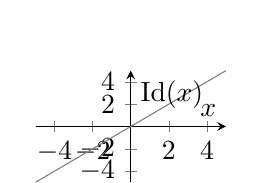
\begin{tikzpicture}
    \begin{axis}[width=4cm, height=3cm, axis lines=middle, xlabel=$x$, ylabel=$\text{Id}(x)$, samples=100]
        \addplot[gray, domain=-5:5] {x};
    \end{axis}
\end{tikzpicture} \\
\hline
Skok Jednostkowy & $\text{Skok}(x) = \begin{cases} 0 & \text{if } x < 0 \\ 1 & \text{if } x \geq 0 \end{cases}$ & 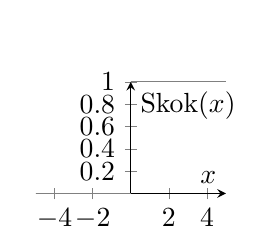
\begin{tikzpicture}
    \begin{axis}[width=4cm, height=3cm, axis lines=middle, xlabel=$x$, ylabel=$\text{Skok}(x)$, samples=100]
        \addplot[gray, domain=-5:0, forget plot] {0};
        \addplot[gray, domain=0:5] {1};
    \end{axis}
\end{tikzpicture} \\
\hline
Sigmoida & $\sigma(x) = \frac{1}{1 + e^{-x}}$ & 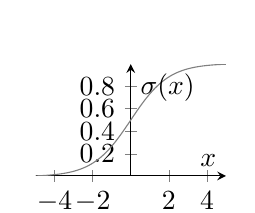
\begin{tikzpicture}
    \begin{axis}[width=4cm, height=3cm, axis lines=middle, xlabel=$x$, ylabel=$\sigma(x)$, samples=100]
        \addplot[gray, domain=-5:5] {1/(1+exp(-x))};
    \end{axis}
\end{tikzpicture} \\
\hline
Tangens Hiperboliczny (tanh) & $\tanh(x) = \frac{e^{x} - e^{-x}}{e^{x} + e^{-x}}$ & 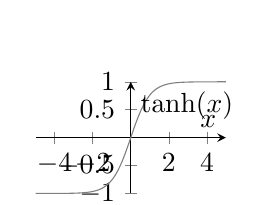
\begin{tikzpicture}
    \begin{axis}[width=4cm, height=3cm, axis lines=middle, xlabel=$x$, ylabel=$\tanh(x)$, samples=100]
        \addplot[gray, domain=-5:5] {(exp(x)-exp(-x))/(exp(x)+exp(-x))};
    \end{axis}
\end{tikzpicture} \\
\hline
ReLU & $\text{ReLU}(x) = \max(0, x)$ & 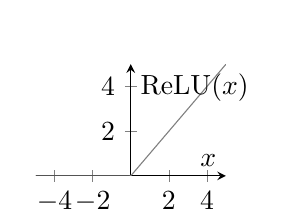
\begin{tikzpicture}
    \begin{axis}[width=4cm, height=3cm, axis lines=middle, xlabel=$x$, ylabel=$\text{ReLU}(x)$, samples=100]
        \addplot[gray, domain=-5:5] {max(0,x)};
    \end{axis}
\end{tikzpicture} \\
\hline
GELU & $\text{GELU}(x) = \frac{1}{2}x\left(1 + \tanh\left(\sqrt{\frac{2}{\pi}}(x + 0.044715x^3)\right)\right)$ & 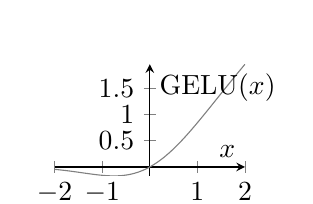
\begin{tikzpicture}
    \begin{axis}[width=4cm, height=3cm, axis lines=middle, xlabel=$x$, ylabel=$\text{GELU}(x)$, samples=100]
        \addplot[gray, domain=-2:2] {0.5*x*(1 + tanh(sqrt(2/pi)*(x + 0.044715*x^3)))};
    \end{axis}
\end{tikzpicture} \\
\hline
ELU & $\text{ELU}(x) = \begin{cases} x & \text{if } x \geq 0 \\ \alpha (e^{x} - 1) & \text{if } x < 0 \end{cases}$ & 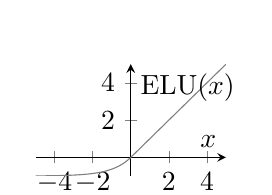
\begin{tikzpicture}
    \begin{axis}[width=4cm, height=3cm, axis lines=middle, xlabel=$x$, ylabel=$\text{ELU}(x)$, samples=100]
        \addplot[gray, domain=-5:5] {ifthenelse(x>=0,x,1*(exp(x)-1))};
    \end{axis}
\end{tikzpicture} \\
\hline
Leaky ReLU & $\text{Leaky ReLU}(x) = \begin{cases} x & \text{if } x \geq 0 \\ \alpha x & \text{if } x < 0 \end{cases}$ & 
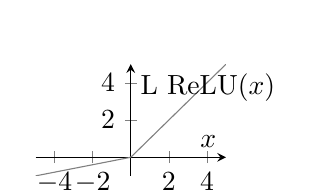
\begin{tikzpicture}
    \begin{axis}[width=4cm, height=3cm, axis lines=middle, xlabel=$x$, ylabel=$\text{L ReLU}(x)$, samples=100]
        \addplot[gray, domain=-5:5] {ifthenelse(x>=0,x,0.2*x)};
    \end{axis}
\end{tikzpicture} \\
\hline
Rozkład Gaussa & $\text{Gauss}(x) = e^{-x^2}$ & 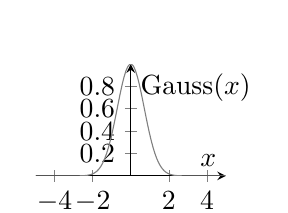
\begin{tikzpicture}
    \begin{axis}[width=4cm, height=3cm, axis lines=middle, xlabel=$x$, ylabel=$\text{Gauss}(x)$, samples=100]
        \addplot[gray, domain=-5:5] {exp(-x^2)};
    \end{axis}
\end{tikzpicture} \\
\hline
Softplus & $\text{Softplus}(x) = \ln(1+e^x)$ & 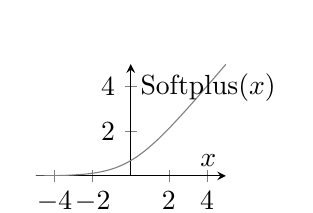
\begin{tikzpicture}
    \begin{axis}[width=4cm, height=3cm, axis lines=middle, xlabel=$x$, ylabel=$\text{Softplus}(x)$, samples=100]
        \addplot[gray, domain=-5:5] {ln(1+exp(x))};
    \end{axis}
\end{tikzpicture} \\
\hline

\end{longtable}

 

\subsection{Perceptrony wielowarstwowe}
\label{sec:NNArchitecture}
Podstawową i najprostszą jednokierunkową siecią neuronową jest perceptron wielowarstwowy MLP \en{multilayer perceptron}. 
Budowę tej sieci konstytuują połączone ze sobą neurony  organizowane w pełni połączone warstwy. Każde dwie sąsiadujące warstwy tworzą ze sobą skierowany i pełny graf dwudzielny z wagami, w którym węzły reprezentowane są przez neurony. Każdy neuron odbiera sygnał od neuronów połączonych z nim w poprzedniej warstwie, a następnie z wykorzystaniem nieliniowej funkcji wyznacza wyjście do kolejnej warstwy na podstawie sumy wejść. Połączenia zwykle mają wagi aktualizowane w procesie uczenia, które wpływają na wartość przepuszczanego sygnału. Sygnał na wejściu sieci jest modyfikowany przez nią, a następnie zwracany w ostatniej warstwie. Przyjęło się nazywać sieci neuronowe \textit{głębokimi} gdy posiadają co najmniej dwie \textit{ukryte} warstwy. Schemat MLP przedstawiono na rys. \ref{fig:MLP}.

\par
Perceptron wielowarstwowy można opisać formalnie za pomocą złożenia funkcji opisującej przekształcenia dokonywane na kolejnych warstwach.
Formalnie, każdą warstwę ukrytą zdefiniować można funkcją w sposób następujący:
\[f_i(x_{i-1})=\sigma(W_i^Tx_{i-1}+b_i)\]
gdzie $\sigma : \mathbb{R} \rightarrow \mathbb{R}$ jest nieliniową funkcją aktywacji, $b_i$ jest wektorem wyrazów wolnych, a $W_i$ macierzą wag. 
\par
Sieć wówczas jest złożeniem funkcji $f_i$ każdej warstwy ukrytej:
\[\phi=f_k\circ \dots \circ f_1\]

A jej warstwa wyjściowa definiowana jest przez wzór:
\[\hat{y}=W^T_o\phi(x)+b_o\]
gdzie $\hat{y}$ odpowiedzią sieci\cite{matematyk2022-fh}. 
\addImage{fig:MLP}{src/img/TheoreticalIntroduction/mlp.png}{Organizacja sieci MLP}

\subsection{Splotowe sieci neuronowe}
\label{sec:cnn}
Splotowe sieci neuronowe są typem jednokierunkowej sieci neuronowej, w której w procesie uczenia optymalizuje się parametry filtrów. Sieci te zakładają wewnętrzne uporządkowania danych wejściowych. Tym samym silną korelację pomiędzy pobliskimi elementami wejścia\cite{lecun1998gradient}. Szczegóły reprezentacji danych przedstawione są poniżej, w rozdziale \ref{sec:imgRepresentation}.
\subsubsection{Reprezentacja obrazu}
\label{sec:imgRepresentation}
\par
Każdy obraz możemy reprezentować jako pewną macierz, której współczynniki opisują w sposób numeryczny wartość piksela, a wzajemne ułożenie elementów macierzy przenosi informację o rozkładzie pikseli na obrazie. W przypadku podstawowych modeli kolorów takich jak RGB, macierz złożona jest z trzech komponentów odpowiadających barwom R - czerwona, G - zielona, B - niebieska, reprezentowanych przez dodatkowy wymiar, zwany \textit{kanałem}. Uogólnienie macierzy z dwóch na dowolną liczbę wymiarów nazywamy tensorem. W przypadku obrazu w skali szarości obraz przechowywany jest przez jeden kanał\cite{zhong2016overview}. 
\par 
W przypadku uczenia sieci MLP do analizy obrazów, obraz wejściowy poddaje się spłaszczeniu \en{flattening}. W przypadku tensora $H=[h_{ijk}]$, gdzie $i \in \{x \in \mathbb{Z}_+ \ | \ x <h \}$, $j \in \{x \in \mathbb{Z}_+ \ | \ x <w \}$,  $k \in \{x \in \mathbb{Z}_+ \ | \ x <c \}$, gdzie $h,w,c$ wysokość obrazu, szerokość obrazu, ilość kanałów odpowiednio, otrzymuje się wektor o wielkości $L=hwc$.
\addImage{fig:flattening}{src/img/TheoreticalIntroduction/flattening.png}{Spłaszczenie tensora do reprezentacji wektorowej}
\par
Sieci MLP jednak mają istotną wadę w rozwiązywaniu problemów wizji komputerowej. W przypadku nawet małych obrazów wielkości 128x128x3 pojedynczy neuron miałby 49153 parametry (łącznie z wyrazem wolnym). Ponieważ sieć złożona jest z wielu neuronów, ilość parametrów jest olbrzymia. Wraz ze zwiększeniem rozdzielczości obrazu ilość parametrów rośnie w sposób kwadratowy. Problem ten nazwany został przekleństwem wymiarowości. Ponadto spłaszczenie obrazu powoduje zanik łatwych korelacji pomiędzy bliskimi pikselami. W procesie uczenia sieć może się nauczyć takich korelacji, jednak wymaga to wiele czasu i olbrzymiej ilości danych\cite{matematyk2022-fh}. Dlatego współcześnie rzadko korzysta się się z sieci MLP celem analizy obrazu. Lepszym podejściem okazują się sieci splotowe. 


\subsubsection{Filtry splotowe}
\label{sec:convolutionalFilters}
Splot jest przekształceniem zdefiniowanym na dwóch funkcjach:
\[(f*g)(t):=\int_{-\infty}^{\infty}f(\tau)g(t-\tau)d\tau\]
\par
Dyskretny splot, używany często w przekształceniach obrazów, definiuje się wzorem\cite{matematyk2022-fh}:
\[g_{xy}=\sum_{i,j,k}h_{ijk}w_{x+i,y+j,k}\]
gdzie 
$W=[w_{ijk}]$ jest tensorem definiującym filtr. Zazwyczaj wymiary filtra są dużo mniejsze niż wymiary obrazu. Splot zachowuje pierwotną informację przestrzenną. Przedstawiono go na rys. \ref{fig:convolution}.

\addImage{fig:convolution}{src/img/TheoreticalIntroduction/convolution.png}{Działanie filtra splotowego. Filtr W jest przykładany do każdego piksela obrazu H otrzymując nową wartość w pikselu, zależną również od początkowego otoczcenia wyrazu}

\subsubsection{Operacja redukująca}
Operacja redukująca \en{pooling} jest najczęściej przeprowadzana z wykorzystaniem filtrów maksymalizujących, który wydobywa maksymalną aktywację z danego pola percepcji. Wówczas nazywana jest \en{max-pooling}. Filtr maksymalizujący ten można przedstawić w następujący sposób:
\[g_{xy}=\max{h_{x \pm i, y \pm j}}\]
gdzie $I,J$ - wymiary filtra, $i \in I, j \in J$. W przypadku wielu splotowych sieci neuronowych filtr ten stosuje się do wybranych elementów obrazu, redukując tym samym jego wymiary, co przekłada się na zmniejszenie złożoności obliczeniowej w procesie uczenia, ograniczenie liczby parametrów i mniejsze zużycie pamięci, a to z kolei ogranicza nadmierne dopasowanie. Stosuje się do tego krok \en{stride}. Jeśli krok równy jest 2x2 to znaczy że do co drugiego piksela w pionie i poziomie przykłada się filtr. 
Operację redukującą przedstawia się na rys \ref{fig:maxpool}.
\addImage{fig:maxpool}{src/img/TheoreticalIntroduction/maxpool.png}{Operacja redukująca max-pool, z wielkością filtra 2x2 i krokiem 2x2}
\par
Wraz z przykładaniem filtra stosuje się również operację dopełnienia \en{padding}. Ma to na celu rozwiązanie problemu z krańcowymi pikselami do których nie można przyłożyć filtra, bo zakres indeksów wykracza poza zakres obrazu. Stosuje się zazwyczaj tzw. zero-padding, czyli dodaje się odpowiedni margines do obrazu wejściowego złożonego z zer. Stosuje się również czasami no-padding, czyli po prostu ignoruje się przyłożenie filtra do skrajnych pikseli (rys. \ref{fig:maxpool}).




\subsubsection{Architektura sieci splotowych}
W sieciach splotowych optymalizuje się wzorce (parametry filtra), tak aby możliwie dobrze rozwiązywały postawione zadanie. Sieć jest podtypem jednokierunkowych sieci neuronowych więc składa się z warstwy wejściowej, warstw ukrytych i warstwy wyjściowej. Wśród warstw ukrytych znajdują się warstwy splotowe \en{convolutional layars} i redukujące \en{pooling layers}.
\par

\begin{description}
    \item[Warstwa splotowa]  
    Zawiera zestaw filtrów, które przekształcają otrzymany obraz. Parametry filtrów podlegają procesowi uczenia. Po każdej warstwie splotowej otrzymywany jest obraz $H_m$, z których ostatni stanowi wysokopoziomową reprezentację początkowego obrazu. Do wyjścia stosuje się funkcję aktywacji wprowadzającą nieliniowość do procesu. W przypadku klasycznego problemu klasyfikacyjnego obraz rzutuje się do przestrzeni klas. Na wyjściu warstwy otrzymywany jest obraz\cite{matematyk2022-fh}:
    \[H_1=f(H*W_1), \dots, f(H*W_l)\]
    \item[Warstwa redukująca]
    Z wykorzystaniem operacji redukującej, zmniejsza wymiarowość danych, co jest często niezbędne aby zredukować złożoność obliczeniową procesu treningowego. Tym samym warstwa ta pełni rolę próbkowania sygnału wejściowego \en{downsampling}.
\end{description}
\par 

Filtr $W_j$ przyłożony do piksela o indeksie $(i,j)$ obrazu $H$ jest utożsamiany z neuronem, w którym wagi są parametrami filtra. W sieci splotowej wagi neuronu nie są połączone ze wszystkimi neuronami z poprzedniej warstwy, ale z pikselami w ich polach percepcyjnych. Ponieważ wagi są współdzielone, zachodzi redukcja w ilości parametrów sieci w zestawieniu z sieciami w pełni połączonymi jak MLP.
\par
W przetwarzaniu danych splot posiada ważne zalety w zestawieniu z klasycznymi metodami używanymi w sieciach w pełni połączonych. Są to lokalność połączeń, wspólne wartości wag połączeń filtru, a na skutek tego niezmienniczość (ekwiwariancja) względem przesunięcia\cite{osowski2018glkebokie}, a więc i lepszą generalizacja. Najprostszym przykładem ekwiwariancji byłby przykład, kiedy ucząc sieć w zbiorze uczącym, wykrywany obiekt występował tylko na pewnym miejscu obrazu. Dla sieci FC w momencie przedstawienia jej nowej danej z tym samym obiektem, lecz w innym miejscu niż w zbiorze uczącym, rzeczone dwa obiekty są różne. W przypadku sieci splotowych, w których używa się filtrów niezależnych od położenia, problem jest znacznie prostszy. Sieć ta posiada większą zdolność generalizacji.


\subsection{Uczenie sieci neuronowych}
W procesie uczenia niezbędne jest posiadanie wystarczającej ilości danych, podzielonych w zbiór uczący, ewaluacyjny i testowy. Do uczenia wykorzystuje się zbiór uczący, natomiast w procesie tym również używa się mniejszego zbioru ewaluacyjnego. W wielu wypadkach w procesie uczenia do warstw podaje się serie danych \en{batch}.
\par
Pierwszym krokiem uczenia nadzorowanej sieci neuronowej jest przepuszczenie danych przez model, obliczając wyjścia poszczególnych warstw ukrytych, a następnie wyjście z sieci. Jest to nazywane krokiem jednokierunkowej sieci \en{feedforward step}. Oblicza się błąd całkowity sieci wykorzystując funkcję kosztu opisaną w szczegółach w rozdziale \ref{sec:cost}. Następnie dla każdej wagi oblicza się pochodną błędu i waga jest aktualizowana przez ujemny czynnik pochodnej. Obliczanie pochodnych  pobudzeń poprzedniej warstwy możliwe, znając pochodne z następnej warstwy. Proces obliczania pochodnych błędu w kolejnych warstwach nazywany jest propagacją wsteczną \en{backpropagation}\cite{lecun1988theoretical}. 
\par
Proces ten powtarzany jest wielokrotnie, każda sesja ucząca jest nazywana epoką \en{epoch}. Zwykle w procesie uczenia po każdej eposze ewaluuje się model na osobnym zbiorze danych, zwanych zbiorem ewaluacyjnym. Ewaluacje klasyfikatorów binarnych opisane zostały w rozdziale \ref{sec:evaluation}. Ma to na celu ochronę procesu uczenia przed nadmiernym dopasowaniem oraz ocenę jakości uczenia oraz modelu.  
\subsubsection{Funkcja kosztu}
\label{sec:cost}
Funkcja kosztu jest kryterium jakości znalezionego rozwiązania. Dlatego problem minimalizacji (optymalizacji) funkcji kosztu jest kluczowym zagadnieniem uczenia maszynowego. W przypadku prostych funkcji możliwe jest znalezienie rozwiązania analitycznego, jednak w większości przypadków stosuje się numeryczne schematy minimalizacji.
\par 
W przypadku uczenia nadzorowanego funkcje kosztu przyjmują na wejście dane predykcji, czyli wyjścia, oraz dane rzeczywiste, będące punktem odniesienia i tym są bardziej podobne do siebie, tym zwracana wartość funkcji kosztu jest mniejsza. 
\par Przykładowymi funkcjami kosztu są:


\begin{longtable}{p{0.3\textwidth}p{0.6\textwidth}}
    \caption{Funkcje kosztu}
    \label{tab:loss_functions} \\
    \toprule
    \textbf{Funkcja Straty (Równanie)} & \textbf{Opis} \\
    \midrule
    \endfirsthead
    
    \multicolumn{2}{c}{{\tablename\ \thetable{} -- Kontynuacja z poprzedniej strony}} \\
    \toprule
    \textbf{Funkcja Straty (Równanie)} & \textbf{Opis} \\
    \midrule
    \endhead
    
    \midrule
    \multicolumn{2}{r}{{Kontynuacja na następnej stronie}} \\
    \endfoot
    
    \bottomrule
    \endlastfoot
    
    \textbf{Błąd średniokwadratowy (MSE)} & 
    \( \text{MSE} = \frac{1}{n} \sum_{i=1}^{n} (y_i - \hat{y}_i)^2 \) \\
    & Mierzy średnią kwadratową różnicy między prognozami modelu a rzeczywistymi wartościami. Jest często używana w problemach regresji. \\
    \hline
    \textbf{Binarna entropia krzyżowa (BCE)} & 
    \( \text{BCE} = -\frac{1}{n} \sum_{i=1}^{n} \left[ y_i \cdot \log(\hat{y}_i) + (1 - y_i) \cdot \log(1 - \hat{y}_i) \right] \) \\
    & Stosuje się ją w problemach klasyfikacji binarnej. BCE mierzy entropię krzyżową pomiędzy rzeczywistymi i przewidywanymi rozkładami prawdopodobieństwa. Jest szczególnie skuteczna w zadaniach binarnej klasyfikacji, jednak czasami nie radzi sobie z trudnymi przypadkami. \\
    \hline
    \textbf{Hinge} & 
    \( \text{Hinge Loss} = \max(0, 1 - y \cdot f(x)) \) \\
    & Powszechnie stosowana w uczeniu maszynowym dla problemów klasyfikacji SVM (maszyn wektorów nośnych). \\
    \hline
    \textbf{Huber} & 
    \( \text{Huber Loss} = \begin{cases} \frac{1}{2} \left( y - \hat{y} \right)^2, & \text{dla } |y - \hat{y}| \leq \delta, \\ \delta \cdot \left( |y - \hat{y}| - \frac{1}{2} \delta \right), & \text{dla } |y - \hat{y}| > \delta. \end{cases} \) \\
    & Jest alternatywą dla MSE, bardziej odporną na wartości odstające. \\
     \hline
	\textbf{Focal} & 
	$\begin{aligned}
		&\text{Focal} = -\frac{1}{n} \sum_{i=1}^{n} \bigg[ y_i \cdot (1 - \hat{y}_i)^\gamma \cdot \log(\hat{y}_i) + \\
		& \qquad \qquad (1 - y_i) \cdot \hat{y}_i^\gamma \cdot \log(1 - \hat{y}_i) \bigg]
	\end{aligned} $\\
	& Wprowadza czynnik modyfikujący \(\gamma\), aby zminimalizować wpływ poprawnie sklasyfikowanych przykładów. Skuteczna w radzeniu sobie z problemem nierówności klas w zadaniach klasyfikacji\cite{Lin_2017_ICCV}. \\
	
	%	\( \text{FL} = -(1-p_t)^\gamma\log{p_t}\) \\ 
	
    
    
\end{longtable}


\subsubsection{Optymalizacja}
\label{sec:optimization}
\par
Optymalizacja jest procesem wykorzystującym spadek gradientu celem znalezienia lepszego rozwiązania problemu. Opisane zostaną dwa algorytmy  optymalizacyjne: metoda stochastycznego gradientu prostego oraz optymalizator Adam.
\\

\textbf{Stochastyczna metoda gradientu prostego (SGD)} jest podstawowym algorytmem optymalizacji stosowanym w procesie uczącym modeli uczenia maszynowego. Algorytm ten jest wrażliwy na dobór hiperparametrów, w szczególności kroku uczenia $\eta$. Może on bardzo silnie wpłynąć na proces uczenia i rozwiązanie. Mały krok może wpływać na bardzo powolne tempo procesu uczenia, zbyt duży krok na rozbieżność tegoż. Poniżej znajduje się opis SGD.


\begin{enumerate}
    \item Inicjalizacja parametrów: Algorytm rozpoczyna się od losowej inicjalizacji wag modelu.
    
    \item Przygotowanie danych: W każdej iteracji algorytmu losowo wybiera podzbiór danych treningowych (batch) do obliczenia gradientu funkcji kosztu.
    
    \item Obliczenia gradientu: Na podstawie wybranego batcha danych oblicza się gradient funkcji kosztu względem parametrów modelu.
    
    \item Aktualizacja parametrów: Wagi modelu są aktualizowane zgodnie z równaniem:
    \begin{equation*}
        \theta_{t+1} = \theta_t - \eta \cdot \nabla J(\theta_t),
    \end{equation*}
    gdzie \(\theta_t\) to parametry modelu w iteracji \(t\), \(\eta\) to krok uczenia, a \(\nabla J(\theta_t)\) to gradient funkcji kosztu.
    
    \item Iteracje: Proces iteracyjny powtarza się dla każdego batcha danych aż do osiągnięcia warunku zakończenia, na przykład określonej liczby epok.
\end{enumerate}

\par
    

\textbf{Adam} (Adaptive Moment Estimation) to zaawansowany algorytm optymalizacji używany w treningu modeli uczenia maszynowego, będący niejako odpowiedzią na słabości SGD\cite{kingma2014adam}. Optymalizator zakłada wykorzystanie momentum\cite{rumelhart1986learning}, czyli elementu pamiętającego aktualizację uczenia z poprzednich iteracji algorytmu. Nie posiada stałego kroku uczenia, jest rodzajem optymalizatora adaptacyjnego. Złożony jest z następujących kroków:


\begin{enumerate}
    \item Inicjalizacja parametrów: Adam inicjalizuje moment pierwszego rzędu \(m\) i moment drugiego rzędu \(v\) dla każdego parametru modelu. Inicjalizuje się również licznik iteracji \(t\).
    
    \item Obliczenia gradientu: W każdej iteracji algorytmu oblicza się gradient funkcji celu względem parametrów modelu.
    
    \item Aktualizacja momentu pierwszego rzędu:
    \begin{equation*}
        m_t = \beta_1 \cdot m_{t-1} + (1 - \beta_1) \cdot \nabla_{\Theta}L,
    \end{equation*}
    gdzie \(\nabla_{\Theta}L\) to gradient w aktualnej iteracji, a \(\beta_1\) to współczynnik wygładzania (często bliski 1, na przykład 0.9).
    
    \item Aktualizacja momentu drugiego rzędu:
    \begin{equation*}
        v_t = \beta_2 \cdot v_{t-1} + (1 - \beta_2) \cdot \nabla_{\Theta}L^2,
    \end{equation*}
    gdzie \(\nabla_{\Theta}L^2\) to kwadrat gradientu.
    
    \item Korekta obciążenia momentów: Korektę momentu pierwszego rzędu \(\hat{m}_t\) i momentu drugiego rzędu \(\hat{v}_t\) oblicza się stosując:
    \begin{equation*}
        \hat{m}_t = \frac{m_t}{1 - \beta_1^t}, \quad \hat{v}_t = \frac{v_t}{1 - \beta_2^t}.
    \end{equation*}
    
    \item Aktualizacja parametrów modelu:
    \begin{equation*}
        \theta_{t+1} = \theta_t - \frac{\eta}{\sqrt{\hat{v}_t} + \epsilon} \cdot \hat{m}_t,
    \end{equation*}
    gdzie \(\eta\) to współczynnik uczenia, a \(\epsilon\) to mała, dodatnia stała zapobiegająca dzieleniu przez zero.
\end{enumerate}
\par 


\subsubsection{Regularyzacja}
Celem regularyzacji jest uniknięcie nadmiernego dopasowania. Powstało wiele technik regularyzacyjnych, wśród których wymienić można regularyzację wag, wczesne kończenie procesu treningowego, oraz zastosowanie warstwy porzucenia \en{dropout} oraz batch-normalizacji.
\par
Celem normalizacji jest uzyskanie na każdej współrzędnej średniej bliskiej 0 oraz odchylenia standardowego równego 1. Normalizuje się nie tylko dane wejściowe ale i dane w poszczególnych warstwach sieci, gdyż niektóre aktywacje mogą być dużo większe od innych. W przypadku batch-normalizacji normalizuje się dane wewnątrz serii (batcha). Normalizacja ta pomaga w utrzymaniu stabilności uczenia się, zwłaszcza w przypadku głębokich sieci neuronowych, oraz pozwala na zminimalizowanie problemu zanikających gradientów.
\par
Formalnie batch-norlamizaję możemy opisać następująco:
\par
Oznaczmy \(B\) batch, a średnią i wariancję $B$ jako wektory $\mu_B, \sigma_B^2$. Wówczas proces batch-normalizacji można opisać za pomocą następujących kroków:

\begin{enumerate}
    \item Obliczenie średniej \(\mu_B\) i wariancji \(\sigma_B^2\) batcha:
    \begin{equation*}
        \mu = \frac{1}{|B|} \sum_{x \in B}x x_i, \quad \sigma^2_B = \frac{1}{|B|} \sum_{x \in B} (x - \mu_B)^2.
    \end{equation*}
    
    \item Znormalizowanie danych:
    \begin{equation*}
        \hat{x} = \frac{x - \mu_B}{\sqrt{\sigma^2_B + \epsilon}},
    \end{equation*}
    gdzie \(\epsilon\) to mała dodatnia stała zapobiegająca dzieleniu przez zero, a $x \in B$
    
    \item Skalowanie i przesunięcie danych:
    \begin{equation*}
        y = \gamma \hat{x} + \beta,
    \end{equation*}
    gdzie \(\gamma\) to parametr skalowania, pozwalający dostosować odchylenie standardowe a \(\beta\) to parametr przesunięcia, pozwalający regulować wyraz wolny (bias). Oba parametry podlegają procesowi uczenia\cite{ioffe2015batch}.
\end{enumerate}
\clearpage

\section{Metodyka badawcza i użyte technologie}
\subsection{Dobór zbioru danych}
\label{sec:DatasetSelection}
\par
Przez zbiór danych rozumie się skany MRI mózgu oraz odpowiadające im maski, czyli oznaczenia zmian chorobowych dokonane przez lekarza i służące jako obiektywnie prawdziwa wartość oczekiwana do procesu uczenia. Przykładowy element w modalności FLAIR został przedstawiony na obrazie rys. \ref{fig:DBInstance-scheme}. \addImage{fig:DBInstance-scheme}{src/img/ScientificMethodsAndTechnology/DBInstance-scheme-bw.png}{Przykładowa instancja danej w zbiorze danych}.
\par
Na zbiór danych składa się 97 trójwymiarowych skanów MRI mózgu zapisanych w standardzie nifti. Każdy z obrazów jest wielkości ok. 200x200x200 pikseli, a poszczególne różnią się od siebie rozmiarem. Przekłada się to na 22 115 przekrojów poprzecznych mózgu. Zbiór danych został pozyskany z dwóch źródeł\cite{malinin2022shifts}. 
\par 
Pierwszym z nich jest Observatoire Français de la Sclérose en Plaques (OFSEP), będące francuskim rejestrem MS, stworzonym dzięki powszechnym wykorzystaniu Europejskiej bazy danych stwardnienia rozsianego (EDMUS)\cite{Vukusic2020-mg}\cite{Confavreux1992-em}. OFSEP w 2018 roku był w posiadaniu 68 097 plików, z czego 71.1\% stanowiły obrazy mózgów kobiet, co jest reprezentatywne biorąc pod uwagę epidemiologię MS. Dane są publicznie dostępne dla potrzeb naukowych. Wszystkie dostępne zostały wykonane w Rennes, Bordeaux i Lyon skanerami 3.0T Siemens Verio, GE Discovery i Philips Ingenia oraz 1.5T Siemens Aera. Obrazy masek powstały na zasadzie konsensusu 7 lekarzy oznaczających lezje. Z powyższego zbioru zostało pobranych 52 trójwymiarowe skany mózgu. 
\par
Drugim źródłem danych jest dostępna na publicznej licencji  Creative Commons CC BY-NC-SA 4.0 kombinacja zbiorów ISBI pobranych w Best\cite{Carass2017-xz}\cite{Carass2017-al} oraz PubMRI w Ljubljanie\cite{Lesjak2018-vo}. Na dane składają się 47 skany mózgów, otrzymanych za pomocą 3.0T tomografów Philips Medical oraz Siemens Magnetom Trio. Maski zostały określone przez konsensus trzech lekarzy w przypadku danych z Ljublany i dwóch w przypadku danych z Best. 
\par Rozdzielczość pobranych obrazów została przedstawiona w tabeli \tabRef{tab:ResolutionOfDataset}.

\begin{table}[H]
    \centering
    \caption{Rozdzielczość skanerów wykorzystanych do tworzenia zbioru danych}
    \begin{tabular}{|c|c|c|c|}
    \hline
    Lokacja & Skaner & Pole & Rozdzielczość \\
    \hline
    Rennes - OFSEP & Siemens Verio & 3.0T & $0.50 \times 0.50 \times 1.10$  \\
    \hline
    Bordeaux - OFSEP & GE Discovery & 3.0T & $0.47 \times 0.47 \times 0.90$  \\

    & Siemens Aera & 1.5T & $1.03 \times 1.03 \times 1.25$  \\
    \hline
    Lyon - OFSEP & Philips Ingenia & 3.0T & $0.74 \times 0.74 \times 0.70$  \\
    \hline
    Best - ISBI & Philips Medical & 3.0T & $0.82 \times 0.82 \times 2.20$  \\
    \hline
    Ljubljana - PubMRI & Siemens Magnetom Trio & 3.0T & $0.47 \times 0.47 \times 0.80$  \\
    \hline
    \end{tabular}
    \label{tab:ResolutionOfDataset}
\end{table}

\par 
Wszystkie dane używane w pracy zostały poddane procesowi anonimizacji przez ich dostawcę.  
Wszystkie zbiory zostały pozyskane z legalnych źródeł i traktowane według licencji na których zostały udostępnione.




\subsection{Dobór środowiska programistycznego}
\label{sec:IDESelection}
\par
Do realizacji zadania wybrano DataSpell 2023.1.2, zintegrowane środowisko programistyczne (IDE) firmy JetBrains służące do obsługi skryptów języka Python, notatników Jupyter, mająca ułatwiać realizację zagadnień danologii. IDE wspiera edycję i analizę kodu źródłowego, posiada graficzny debuger, pozwala na wykorzystanie jądra Linuxowego przez warstwę kompatybilności Windows Subsystem for Linux (WSL 2) dla użytkowników systemu Windows oraz umożliwia integrację z systemem kontroli wersji. Ponadto przez wygodny interfejs użytkownika pozwala na korzystanie z systemów zarządzania pakietami dla środowiska języka Python. Środowisko DataSpell jest częścią szerokiego i uznanego ekosystemu środowisk programistycznych stworzonych przez JetBrains. 
\par 
Do realizacji zadań na Google Colab stosuje się edytor dostępny dla tej usługi, jednakże jedynie celem modyfikacji notatników. Z wykorzystaniem kontroli wersji zintegrowanej z repozytorium w chmurze, notatnik służący do przeprowadzenia procesu uczenia się pobiera niezbędne pakiety. Tym samym, sama modyfikacja kodu źródłowego jest wykonywana w dalszym ciągu przy wykorzystaniu DataSpell, a łącznikiem jest repozytorium w chmurze.

\subsection{Dobór graficznej jednostki obliczeniowej (GPU)}
\label{sec:GPUSelection}
\begin{table}[H]
    \centering
    \caption{ Porównanie specyfikacji jednostek graficznych}
    \begin{tabular}{c|c|c}
    % \hline
    & GeForce RTX 3060 Ti\footnotemark[1] & Turing Tesla T4\footnotemark[2]\\
    \hline
    Liczba rdzeni NVIDIA CUDA & 4864 & 2560  \\
    \hline
    Częstotliwość podwyższona (GHz) & 1,67 &  1,59\\
    \hline
    Częstotliwość bazowa (GHz) & 1,41  & 0,585\\
    \hline
    Standardowa konfiguracja pamięci & 8 GB GDDR6 & 16 GB GDDR6  \\
    \hline
    Szerokość magistrali pamięci & 256-bitowa  & 256-bitowa\\
    % \hline
    \end{tabular}
    \label{tab:RTX3060TiSpecification}
\end{table}
\par 
Przyjęta architektura, opisana w sekcji \ref{sec:ModelSelection}, wymaga dużych mocy obliczeniowych celem wykonania w sprawny sposób procesu uczenia maszynowego. Odpowiadając na wymagania funkcjonalne opisane w \ref{sec:NetworkRequirements}, przyjęto wykorzystanie technologii general-purpose computing on graphics processing units (GPGPU) do przeprowadzenia obliczeń równoległych. W tym celu wybrano Compute Unified Device Architecture (CUDA), czyli API firmy Nvidia, pozwalające użytkownikom na wykorzystanie ich kart graficznych do ogólnych zadań obliczeniowych. 
\par
Zdecydowano się wykorzystać do przeprowadzenia obliczeń procesor GPU NVIDIA GeForce RTX 3060 Ti o specyfikacji wyszczególnionej w tabeli \tabRef{tab:RTX3060TiSpecification}, ze sterownikiem na dystrybucję Ubuntu-WSL, CUDA Toolkit 12.1. 
Pomocniczo zdecydowano wykorzystać procesor GPU Tesla T4 udostępniany przez Google Colab, jako możliwy do wykorzystania w chmurze. Niestety ze względu na duże ograniczenia jakie zostały nałożone na nawet płatne wersje usługi, oraz gorsze parametry jednostki, traktuje się ją drugorzędnie.


\footnotetext[1]{https://www.nvidia.com/pl-pl/geforce/graphics-cards/30-series/rtx-3060-3060ti/}
\footnotetext[2]{https://www.nvidia.com/en-us/data-center/tesla-t4/}


\subsection{Dobór modelu sieci neuronowej}
\label{sec:nn-selection}
\addImage{fig:UNet-scheme}{src/img/ScientificMethodsAndTechnology/UNet-bw.png}{Schemat architektury splotowej sieci neuronowej U-Net}
Przyjęto architekturę U-Net do realizacji zadania. Jest to splotowa sieć neuronowa zaproponowana w 2015 roku przez Departament Nauk Komputerowych Uniwersytetu we Freiburgu\cite{ronneberger2015unet} celem segmentacji na obrazach medycznych. Na architekturę sieci składa się ścieżka kurcząca (lewa strona) i ścieżka rozszerzająca (prawa strona). Pierwsza wygląda jak typowa architektura splotowej sieci, składając się z powtarzających się splotów 3x3, z których po każdym stosuje się rektyfikowaną jednostkę liniową ReLU oraz maskymalizująca warstwa łącząca \en{max pooling layer} 2x2 z krokiem 2. W każdym decymacyjnym kroku podwaja się ilość kanałów cech. W przypadku ścieżki rozszerzającej każdy krok składa się z interpolacji mapy cech, po których następuje splot 2x2, dwukrotnie zmniejszający ilość kanałów cech, konkatenację z przyciętą mapą cech ze ścieżki kurczącej i dwóch splotów 3x3 wraz z ReLU. Według twórców modelu przycinanie jest niezbędne ze względu na utratę pikseli krańcowych podczas splotu. Końcową warstwę buduje splot 1x1 do zmapowania wszystkich 64 cech z oczekiwaną liczbą klas. Schemat sieci U-Net został przedstawiony na rys. \ref{fig:UNet-scheme}.


\par
U-Net jest siecią powszechnie stosowaną w zastosowaniach medycznych. Powstało wiele prac wykorzystujących architekturę U-Net w segmentacji istoty białej oraz szarej \cite{PRZYBYSZEWSKI_KOHUT_2020}, segmentacji guza \cite{Ru2021} oraz zmian chorobowych Alzheimera\cite{Kavitha2019} z dobrymi rezultatami.





\label{sec:ModelSelection}
\subsection{Dobór funkcji kosztu}
\label{sec:choosing-of-cost-function}
\par
Zdecydowano się na dobór entropii krzyżowej z ważeniem na funkcję kosztu. Ważenie zdecydowano się zastosować jako środek zaradczy przeciw dużemu niezbalansowaniu danych, wynoszących w wykorzystywanym zbiorze danych w sumie  1 480 241 pikseli lezji na 590 002 975 pikseli tła. Daje to około 0.25\% oraz 99.75\% pikseli w klasie lezji oraz tła odpowiednio. Zastosowano różne wagi, przede wszystkim wagę klasy lezji 20 oraz 400, w pełni równoważącą niezbalansowanie danych. Postanowiono wykorzystać również funkcję kosztu Focal, również użyteczną w przypadku niezbalansowanych danych.


\subsection{Dobór optymalizatora}
\label{sec:choosing-of-optimizer}
\par
Wybrano optymalizator Adam opisany w rozdziale \ref{sec:optimization}, ze względu na jego zalety adaptacyjne. Testowano również optymalizator SGD, jednak ze znacznie gorszymi rezultatami. Rozważano wykorzystanie innych optymalizatorów adaptacyjnych jak Adagrad, Adadelta, RMSprop. Odrzucono je na rzecz optymalizatora Adam ze względu na uwzględnienie w nich wszystkich, lub wielu, poprzednich gradientów, prowadzące do znacznego zmniejszenia kroku uczenia po pewnym czasie\cite{Haji2021-lj}.

% \subsection{Metryki ewaluacyjne}
% \label{sec:metrics-methodics}
% \par
% Zdecydowano się na użycie wszystkich metryk ewaluacyjnych opisanych w sekcji \ref{sec:confusion-matrix-and-metrics}. 

\subsection{Język programowania Python oraz użyte biblioteki}
\label{sec:pyhton}
\par 
Zdecydowano się na wykorzystanie języka programowania Python, ze względu na liczne biblioteki potencjalnie użyteczne na każdym etapie wykonania zadania oraz prostotę w obsłudze. Python jest powszechnie wykorzystywanym językiem do realizacji projektów z zagadnienia uczenia maszynowego. 
\par 
Jako bibliotekę do uczenia maszynowego wybrano otwartoźródłową \textit{PyTorch 2.0}, stworzoną przez zespół MetaAI. Biblioteka pozwala w łatwy sposób przeprowadzać obliczenia na tensorach, wykorzystując GPU w celu przyspieszenia operacji. Interfejs pozwalający na korzystanie z tensorów podobny jest do interfejsu powszechnie znanej biblioteki \textit{Numpy}. Ponadto posiada automatyczny system do różniczkowania. Posiada również ogromną zaletę w postaci przejrzystego interfejsu oraz w opinii autora, biblioteka pozwala na łatwe wynajdowanie błędów. Zaleta ta, oraz przejrzystość, w dużej mierze była powodem wybrania do realizacji zadania biblioteki \textit{PyTorch}, nad starszą i powszechniejszą biblioteką \textit{TensorFlow} przygotowaną przez Google Brain. Do analizy metryk wykorzystano zintegrowaną z \textit{PyTorch} bibliotekę \textit{TorchMetrics}.
\par 
Wykorzystano również standardowe biblioteki programistyczne jak \textit{pillow, numpy, matplotlib, scikit, scipy, tqdm}, oraz do obsługi plików Nifti bibliotekę \textit{nibabel}.
\clearpage

\tikzstyle{class} = [rectangle, draw, text width=8em, text centered, minimum height=4em, font=\ttfamily]
\tikzstyle{line} = [draw, -latex']

\section{Realizacja}
\label{sec:Execution}
\subsection{Przygotowanie zbioru danych}
\label{sec:preparing-of-dataset}
Do realizacji zadania uznano za konieczne konwersję plików Nifti z rozszerzeniem .nii do plików z rozszerzeniem .npy przechowujących tablice NumPy. Zrobiono tak, ponieważ konwersja do tablic NumPy jest przeprowadzana wielokrotnie podczas procesu uczenia się. Konwersja ta, przy wykorzystaniu biblioteki nibabel, jeśli by wykonywać ją w każdej eposze uczenia, w wymierny sposób spowalniałaby cały proces. Wczytywanie tablic bezpośrednio z plików .npy natomiast usprawnia go. Tablice NumPy są przekrojami poprzecznymi skanów mózgu. Otrzymano w ten sposób 23 281 przekrojów. 
\par 
Wczytywane pliki Nifti początkowo zostają wczytane do klasy \texttt{Nifti}, reprezentującej obraz MRI oraz ewentualnie odpowiadającą mu maskę z oznaczonymi lezjami. Klasa implementuje metodę która w inteligentny sposób przycina obrazy, na podstawie wyznaczonego środka ciężkości na obrazie skanu mózgu. W ten sposób wszystkie obrazy są przestrzennie unormowane.

% \begin{code}
% \begin{minted}[breaklines, linenos]{python}
%     def __intelligent_crop(self):
%         if self.__masks is None:
%             raise Exception("Annotations is {}".format(None))
%         center_of_mass = np.round(ndimage.center_of_mass(np.ceil(self.__images))).astype(int)
%         # Half-length of a maximum possible rectangle side, making center of mass in the center of image.
%         # Take into consideration, that center of mass is the center of gravity for whole 3D image, not just a slice.
%         a = int(min([center_of_mass[1], center_of_mass[2], self.__images.shape[1] - center_of_mass[1], self.__images.shape[2] - center_of_mass[2]]))
%         self.__images = self.__images[:, center_of_mass[1] - a: center_of_mass[1] + a, center_of_mass[2] - a:center_of_mass[2] + a]
%         self.__masks = self.__masks[:, center_of_mass[1] - a: center_of_mass[1] + a, center_of_mass[2] - a:center_of_mass[2] + a]
% \end{minted}
% \captionof{listing}{Wyśrodkowanie obrazu}
% \label{lis:centering-image}
% \end{code}


\subsection{Klasa zbioru danych}
\label{sec:dataset-class}
\par
Celem dostosowania danych do wymagań biblioteki PyTorch niezbędne było stworzenie klasy reprezentującej zbiór danych, pochodnej generycznej klasy \texttt{Dataset} biblioteki. Zdecydowano się na implementację klasy zbioru w stylu mapy, definiowanej przez PyTorch jako definiującą metody \texttt{\_\_len\_\_} oraz \texttt{\_\_item\_\_}. Metody te zwracają ilość elementów w zbiorze danych oraz przekrój mózgu wraz z maską lezji odpowiednio. Klasa implementuje szereg środków zapobiegawczych, mających przeciwdziałać potencjalnej niezgodności danych. 
\begin{figure}[H]
    \centering
    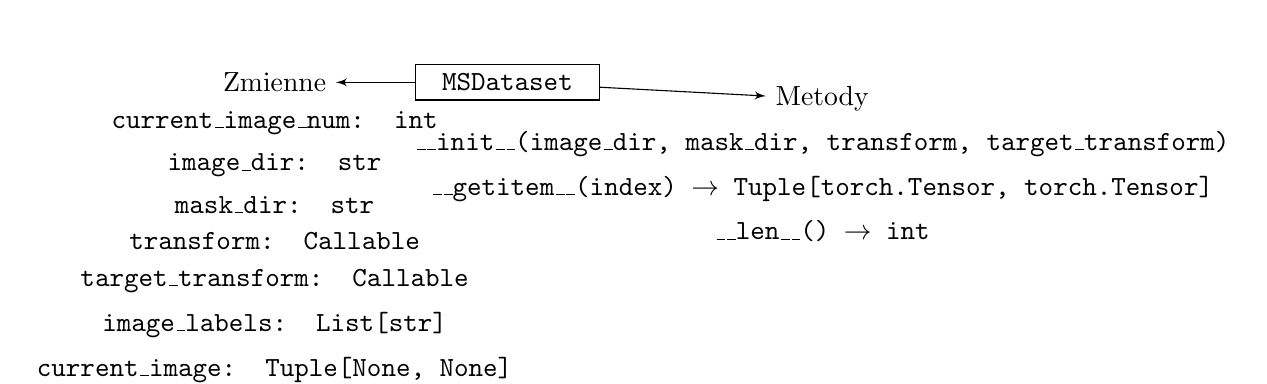
\begin{tikzpicture}[node distance = 0cm, auto,
        class/.style={rectangle, draw, text centered, anchor=north, text width=6em, font=\ttfamily},
        line/.style={draw, -latex'},
        method/.style={font=\ttfamily}
    ]
        % Class node
        \node[class] (dataset) {MSDataset};
        % Private members
        \node[left=1cm of dataset, yshift=0cm] (variables) {\textbf{Zmienne}};
        \node[below=0cm of variables, method] (current_image_num) {current\_image\_num: int};
        \node[below=0cm of current_image_num, method] (image_dir) {image\_dir: str};
        \node[below=0cm of image_dir, method] (mask_dir) {mask\_dir: str};
        \node[below=0cm of mask_dir, method] (transform) {transform: Callable};
        \node[below=0cm of transform, method] (target_transform) {target\_transform: Callable};
        \node[below=0cm of target_transform, method] (image_labels) {image\_labels: List[str]};
        \node[below=0cm of image_labels, method] (current_image) {current\_image: Tuple[None, None]};
        % Public methods
        \node[below=-0.3cm of dataset, xshift=4cm] (methods) {\textbf{Metody}};
        \node[below=0cm of methods, method] (init) {\_\_init\_\_(image\_dir, mask\_dir, transform, target\_transform)};
        \node[below=0cm of init, method] (getitem) {\_\_getitem\_\_(index) $\rightarrow$ Tuple[torch.Tensor, torch.Tensor]};
        \node[below=0cm of getitem, method] (len) {\_\_len\_\_() $\rightarrow$ int};
        % Connections
        \path[line] (dataset) -- (variables);
        \path[line] (dataset) -- (methods);

    \end{tikzpicture}
    \caption{Diagram klasy \texttt{MSDataset}}
    \label{fig:msdataset}
\end{figure}




\subsection{Klasa modelu}
\label{sec:model-class}


\begin{figure}
    \centering
    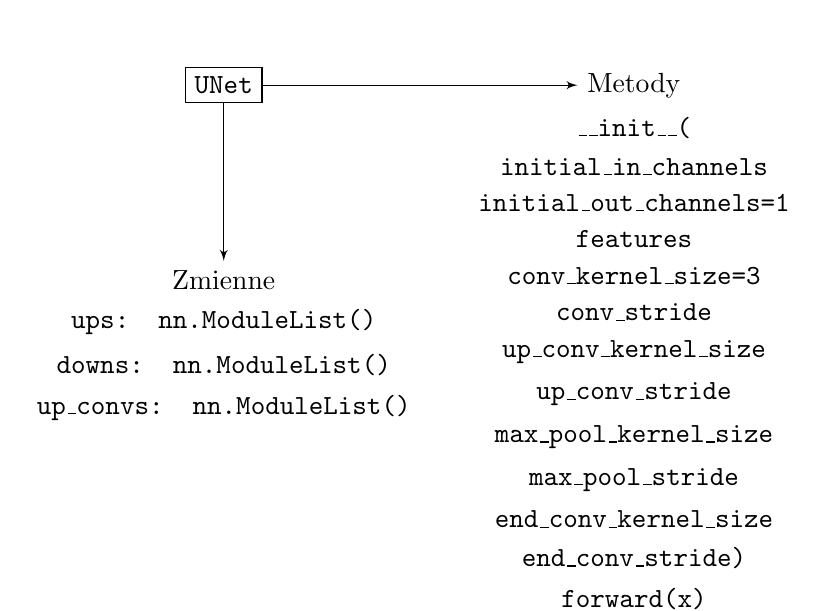
\begin{tikzpicture}[node distance = 0.5cm, auto,
        class/.style={rectangle, draw, text centered, anchor=north, font=\ttfamily},
        line/.style={draw, -latex'},
        method/.style={rectangle, font=\ttfamily}
    ]
        % Class node
        \node[class] (unet) {UNet};
        % Private members
        \node[below=2cm of unet] (variables) {\textbf{Zmienne}};
        \node[below=0cm of variables, method] (ups) {ups: nn.ModuleList()};
        \node[below=0cm of ups, method] (downs) {downs: nn.ModuleList()};
        \node[below=0cm of downs, method] (up_convs) {up\_convs: nn.ModuleList()};
        % Public methods
        \node[right=4cm of unet] (methods) {\textbf{Metody}};
        \node[below=0cm of methods, method] (init) {\_\_init\_\_(};

        \node[below=0cm of init, method] (initial_in_channels) {initial\_in\_channels};
        \node[below=0cm of initial_in_channels, method] (initial_out_channels) {initial\_out\_channels=1};
        \node[below=0cm of initial_out_channels, method] (features) {features};
        \node[below=0cm of features, method] (conv_kernel_size) {conv\_kernel\_size=3};
        \node[below=0cm of conv_kernel_size, method] (conv_stride) {conv\_stride};
        \node[below=0cm of conv_stride, method] (up_conv_kernel_size) {up\_conv\_kernel\_size};
        \node[below=0cm of up_conv_kernel_size, method] (up_conv_stride) {up\_conv\_stride};
        \node[below=0cm of up_conv_stride, method] (max_pool_kernel_size) {max\_pool\_kernel\_size};
        \node[below=0cm of max_pool_kernel_size, method] (max_pool_stride) {max\_pool\_stride};
        \node[below=0cm of max_pool_stride, method] (end_conv_kernel_size) {end\_conv\_kernel\_size};
        \node[below=0cm of end_conv_kernel_size, method] (end_conv_stride) {end\_conv\_stride)};
        
        \node[below=0cm of end_conv_stride, method] (forward) {forward(x)};
        % Connections
         \path[line] (unet) -- (methods);
         \path[line] (unet) -- (variables);
    \end{tikzpicture}
    \caption{Diagram klasy \texttt{UNet}}
    \label{fig:unet}
\end{figure}

Klasa \texttt{nn.Module}  biblioteki PyTorch reprezentuje moduł sieci neuronowej, to jest element który wykonuje pewne obliczenia. Wynik tych obliczeń zwracany jest przy wykorzystaniu metody \texttt{forward}, która to metoda powinna być nadpisana w implementowanym module.  Każdy moduł \texttt{nn.Module} może zawierać inne moduły, w ten sposób tworząc strukturę drzewiastą. W implementacji sieci będącej tematem  tej pracy, w klasie \texttt{UNet}, będącej  modułem \texttt{nn.Module}, stworzono kontener \texttt{nn.Sequential} przechowującym submoduły w sposób sekwencyjny, Kontenery te przyjmują na  wejście dowolne wartości i przekazują je na wejście pierwszego submodułu, w którym następnie obliczane jest wyjście wspomnianą funkcją \texttt{forward} i podawane na wejście kolejnego submodułu. Taka operacja jest powtarzana aż to otrzymania wyjścia z ostatniego submodułu, będącego wyjściem modułu \texttt{nn.Sequential}. W przypadku implementowanej sieci submodułami są między innymi moduły implementujące podwójną konwolucję (przechowującą w istocie element \texttt{nn.Sequential} łączący dwie konwolucje) oraz operacje warstwy redukującej. Schemat klasy przedstawiono na rys. \ref{fig:unet}.

\addImage{fig:unet-class-idea}{src/img/Execution/unet-class.png}{Schemat ideowy działania metody \texttt{forward} klasy \texttt{UNet}}

\par
Pierwszy blok reprezentuje ścieżkę kurczącą, trzeci natomiast reprezentuje ścieżką rozszerzającą. Środkowy blok zawiera elementy ścieżek kurczącej i rozszerzającej i dodany został z powodów praktycznych.
\subsection{Metody uczące}
\par
Zaimplementowano funkcję \texttt{fit} wzorowaną na metodzie \texttt{model.fit()} biblioteki TensorFlow, będącą metodą włączoną do klasy  modelu, ucząc model zadaną ilość epok. Funkcja przygotowana w ramach realizacji zadania jednak nie jest częścią  klasy modelu oraz przyjmuje dodatkowe dane. Wśród nich wyróżnić można uczony model, optymalizatior, funkcję kosztu, skaler. Nie implementowano funkcji jako elementu modelu, trzymając się sensownego w opinii autora ideowego podziału jaki występuje w bibliotece PyTorch, która nie zawiera w modelu  parametrów uczenia.



\par Metoda \texttt{fit} automatycznie wybiera GPU jako jednostkę obliczeniową używaną w procesie uczenia. Tworzy obiekty klasy  \texttt{DataLoader} biblioteki PyTorch obsługującą podawane obrazy i maski lezji do procesu uczenia. Podając do funkcji w argumencie wytrenowany w części model, dano możliwość wznowienia procesu uczenia. Funkcja następnie przeprowadza proces uczenia zadaną w parametrze \texttt{epochs} liczbę razy. Pobierając dane  z obiektów \texttt{DataLoader}, dla każdej serii danych przeprowadza propagację oraz propagację wsteczną wykorzystując obliczone wartości funkcji kosztu. Proces uczenia jest monitorowany przez pasek postępu \texttt{tqdm}. Po przeprowadzeniu każdej sesji uczenia, czyli pod koniec każdej epoki, funkcja \texttt{fit} ewaluuje metryki. Wykorzystuje do tego elementy stworzonej klasy \texttt{MetricsHandler}. Co zadaną w parametrach  wejściowych liczbę epok, funkcja zapisuje stan modelu.




\subsection{Metody ewaluacyjne}
\begin{figure}[H]
	\centering
	\begin{tikzpicture}[node distance = 0cm, auto,
		method/.style={font=\ttfamily}]
		% Class node
		\node[class] (metrics) {Metrics};
		% Private members
		\node[above=2.2cm of metrics, xshift=-4.5cm] (private_members) {\textbf{Prywatne zmienne:}};
		\node[below=0cm of private_members, method] (ppv) {\_\_E\_ppv: float};
		\node[below=0cm of ppv, method] (acc) {\_\_E\_acc: float};
		\node[below=0cm of acc, method] (bacc) {\_\_E\_bacc: float};
		\node[below=0cm of bacc, method] (tpr) {\_\_E\_tpr: float};
		\node[below=0cm of tpr, method] (tnr) {\_\_E\_tnr: float};
		\node[below=0cm of tnr, method] (f05) {\_\_E\_f05: float};
		\node[below=0cm of f05, method] (f1) {\_\_E\_f1: float};
		\node[below=0cm of f1, method] (f2) {\_\_E\_f2: float};
		\node[below=0cm of f2, method] (k) {\_\_E\_k: float};
		\node[below=0cm of k, method] (mcc) {\_\_E\_mcc: float};
		\node[below=0cm of mcc, method] (jacc) {\_\_E\_jacc: float};
		\node[below=0cm of jacc, method] (counter) {\_\_counter: int};
		% Public methods
		\node[above=3.5cm of metrics, xshift=4.5cm] (public_methods) {\textbf{Metody Publiczne:}};
		\node[below=0cm of public_methods, method] (update) {+ update(confusion\_matrix)};
		\node[below=0cm of update, method] (get_counter) {+ get\_counter() $\rightarrow$ int};
		\node[below=0cm of get_counter, method] (ppv_property) {+ ppv() $\rightarrow$ float};
		\node[below=0cm of ppv_property, method] (acc_property) {+ acc() $\rightarrow$ float};
		\node[below=0cm of acc_property, method] (bacc_property) {+ bacc() $\rightarrow$ float};
		\node[below=0cm of bacc_property, method] (tpr_property) {+ tpr() $\rightarrow$ float};
		\node[below=0cm of tpr_property, method] (tnr_property) {+ tnr() $\rightarrow$ float};
		\node[below=0cm of tnr_property, method] (f1_property) {+ f1() $\rightarrow$ float};
		\node[below=0cm of f1_property, method] (f05_property) {+ f05() $\rightarrow$ float};
		\node[below=0cm of f05_property, method] (f2_property) {+ f2() $\rightarrow$ float};
		\node[below=0cm of f2_property, method] (k_property) {+ k() $\rightarrow$ float};
		\node[below=0cm of k_property, method] (mcc_property) {+ mcc() $\rightarrow$ float};
		\node[below=0cm of mcc_property, method] (jacc_property) {+ jacc() $\rightarrow$ float};
		% Connections
		\path[line] (metrics) -- (tnr);
		\path[line] (metrics) -- (tnr_property);
		
	\end{tikzpicture}
	\caption{Diagram klasy \texttt{Metrics}}
	\label{fig:metrics}
\end{figure}
W celu przeprowadzenia ewaluacji modelu stworzono klasy \texttt{Metrics} oraz \texttt{MetricsHandler}. Pierwsza przechowuje przechowuje większość metryk opisanych w rozdz. \ref{sec:confusion-matrix-and-metrics}. Przy wykorzystaniu metody \texttt{update} uaktualnia metryki o nowe dane. Zorganizowano to w podany sposób, gdyż dane podawane są przez \texttt{DataLoader} w seriach i metryki oblicza się dla nich. Klasa \texttt{MetricsHandler} służy do obsługi obliczeń metryk. Do metody inicjacyjnej klasy podawany jest obiekt \texttt{DataLoader}, obsługujący dane ewaluacyjne, obiekt \texttt{nn.Module} przechowujący model, listę \texttt{list} przechowującą wartości progów definiujących przydział do klas końcowych wyjścia modelu, oraz obiekt \texttt{torch.device} określający urządzenie na którym operacje obliczeniowe mają być wykonane. Klasa zawiera metodę \texttt{evaluate}, która zwraca słownik \texttt{dict} z metrykami przyporządkowanymi do konkretnych wartości progów, oraz obliczoną metrykę auroc, jako niezależną od doboru progów. Klasa zawiera również metodę \texttt{append\_metrics} przyjmującą na wejście dwa obiekty \texttt{dict}, która łączy metryki z dwóch słowników i zwraca w postaci jednego słownika \texttt{dict}. Metryki w połączonym słowniku, odpowiadające konkretnym progom (kluczom słownika) są uporządkowane w listę. Metodę tę, używa się obliczając metryki w każdej eposze, w ten sposób otrzymując obiekty \texttt{list} przechowujące metryki dla wielu epoch. Klasa \texttt{MetricsHandler} ponadto posiada wbudowaną metodę do zapisu metryk w formacie .json na dysku.  


\begin{figure}[H]
    \centering
    \begin{tikzpicture}[node distance = 2.5cm, auto,
                method/.style={font=\ttfamily}]
        % Nodes
        \node[class] (handler) {MetricsHandler};
        % Private members
        \node[above left=1.5cm of handler] (private) {\textbf{Zmienne prywatne:}};
        \node[below=0.2cm of private, method] (loader) {\_\_loader: DataLoader};
        \node[below=0.2cm of loader, method] (device) {\_\_device: torch.device};
        \node[below=0.2cm of device, method] (model) {\_\_model: nn.Module};
        \node[below=0.2cm of model, method] (thresholds) {\_\_thresholds: list};
        % Public methods
        \node[below=1.5cm of handler, xshift=-5.5cm] (public) {\textbf{Publiczne metody:}};
        \node[below=0.2cm of public, method] (init) {+ \_\_init\_(loader, model, thresholds, device)};
        \node[below=0.2cm of init, method] (evaluate) {+ evaluate() $\rightarrow$ (threshold\_metric\_dict, b\_auroc\_avg)};
        \node[below=0.2cm of evaluate, method] (append) {+ append\_metrics(to\_append, new\_elements) $\rightarrow$ to\_append};
        \node[below=0.2cm of append, method] (save) {+ save\_metrics(metrics, auroc, path)};
        % Private methods
        \node[below=1.5cm of handler, xshift=2.5cm] (private_methods) {\textbf{Prywatne metody:}};
        \node[below=0.2cm of private_methods, method] (calculate) {- \_calculate\_metrics() $\rightarrow$ dict};
        \node[below=0.2cm of calculate, method] (update) {- \_update\_threshold\_metrics()};
        \node[below=0.2cm of update, method] (save_metric) {- \_save\_metric\_to\_file()};
        % Connections
        \path[line] (handler) -- (device);
        \path[line] (handler) -- (public);
        \path[line] (handler) -- (private_methods);
    \end{tikzpicture}
    \caption{Diagram klasy \texttt{MetricsHandler}}
    \label{fig:metrics-handler}
\end{figure}


\clearpage

\section{Testy i opis wyników}
\label{sec:Tests}
\subsection{Wstęp}

Wytrenowano trzy sieci neuronowe z podanymi parametrami:
\begin{table}[H]
	\centering
	\caption{Parametry uczonych sieci U-Net}
	\begin{tabular}{|c|c|c|c|}
		\hline
		\textbf{} & \textbf{BCE-20} & \textbf{BCE-400} & \textbf{FL-2} \\
		\hline
		\textbf{Optymalizator} & Adam & Adam & Adam \\
		\hline
		\textbf{Funkcja Kosztu} & BCE & BCE & FL \\
		\hline
		\textbf{Ważenie} & 20 & 400 & 2 \\
		\hline
		\textbf{Rozmiar serii (batch)} & 8 & 8 & 8 \\
		\hline
		\textbf{Szybkość uczenia} &1e-4 & 1e-4&1e-4\\
		\hline
		\textbf{Epoki} & 50  & 50 & 50 \\
		\hline
	\end{tabular}
	\label{tab:mytable}
\end{table}
\par
Wszystkie sieci trenowano obrazami wielkości 128x128, rozdzielono zbiór uczący od ewaluacyjnego stosunkiem 4 do 1. Wszystkie zbiory uczące mieszano w procesie uczącym. Zastosowano wszędzie skaler \texttt{GradScaler}. Ważenie odnosi się do klasy mniejszościowej zbioru, tj. przypadków klasyfikacji lezji w BCE-20 i BCE-400. W przypadku FL-2 oznacza ono parametr $\gamma$ funkcji kosztu. Przypomina się, że sumaryczny stosunek pikseli lezji do pikseli tła w zbiorze danych wynosi 1:400, toteż w uczeniu sieci BCE-400 kompletnie balansuje się funkcję kosztu, w przypadku BCE-20 jest ona częściowo zbalansowana. 

\par
Co warto napomnieć, wartość współczynnika F1 obliczana została ze wzoru  $ \mathrm{F_1 = \frac{2\cdot{}|TP|}{2|TP|+|FP|+|FN|}}$ a nie  $\mathrm{2\frac{PPV\cdot{}TPR}{PPV+TPR}}$ W przypadku mianownika równego zero wartość metryki ustalana była arbitralnie na zero, co jest praktyką wykorzystywaną przez większość bibliotek obliczających tą metrykę jak TorchMetrics. Ponieważ mianowniki w obu tych wzorach nie zawsze równocześnie wynoszą zero, to wartości metryk obliczane z obu tych wzorów minimalnie się różnią. Tym samym, obliczona wartość współczynnika Sørensen'a Dice'a nie jest równa średniej harmonicznej z czułości i precyzji. Wykorzystując nauczone modele BCE-20 oraz BCE-400, najlepsze wyniki metryk otrzymano dla progów przypisania do klas wynoszącym 0.9, w przypadku modelu FL-2 najlepsze otrzymano dla progu 0.5.

\subsection{Wytrenowane sieci}
\label{sec:trained-nets}


\subsubsection{BCE-20}

\par
Sieć BCE-20 wykazuje się dobrymi wynikami współczynnika Sørensen'a-Dice'a oraz Jaccarda, oraz najlepsze wyniki współczynnika Kappa spośród wytrenowanych sieci. Uczenie sieci przebiegło w sposób stabilny. Wskaźniki czułości i precyzji również są na wysokim poziomie, osiągając wartość 0.748 oraz 0.912 w ostatniej epoce uczenia.

%\addImage{fig:bce20-2297}{src/img/Tests/bce20-2297.png}{BCE-20 trzy małe lezje}
%\addImage{fig:bce20-4556}{src/img/Tests/bce20-4556.png}{BCE-20 większe lezje}
%\addImage{fig:bce20-9482}{src/img/Tests/bce20-9482.png}{BCE-20 wiele lezji różnych wielkości}





\begin{longtable}[p]{|c|c|c|c|c|c|c|c|c|c|c|c|}
	\caption{Metryki BCE-20} \\
	
	\hline
	\textbf{Epoch} & \textbf{F1} & \textbf{JACC} & \textbf{PPV} & \textbf{TPR} & \textbf{TNR} & \textbf{BACC} & \textbf{K} & \textbf{F05} & \textbf{F2} & \textbf{MCC} \\
	\hline
	\endfirsthead
	
	\multicolumn{11}{c}%
	{{\tablename\ \thetable{} -- Kontynuacja z poprzedniej strony}} \\
	\hline
	\textbf{Epoch} & \textbf{F1} & \textbf{JACC} & \textbf{PPV} & \textbf{TPR} & \textbf{TNR} & \textbf{BACC} & \textbf{K} & \textbf{F05} & \textbf{F2} & \textbf{MCC} \\
	\hline
	\endhead
	
	\hline \multicolumn{11}{|r|}{{Kontynuacja na następnej stronie}} \\ \hline
	\endfoot
	
	\hline
	\endlastfoot
	
	
	1 & 0.612 & 0.459 & 0.517 & 0.781 & 0.998 & 0.880 & 0.477 & 0.569 & 0.775 & 0.601 \\
	2 & 0.652 & 0.501 & 0.557 & 0.809 & 0.998 & 0.894 & 0.523 & 0.624 & 0.792 & 0.659 \\
	3 & 0.639 & 0.495 & 0.822 & 0.546 & 0.999 & 0.763 & 0.488 & 0.586 & 0.757 & 0.568 \\
	4 & 0.707 & 0.564 & 0.640 & 0.805 & 0.999 & 0.892 & 0.591 & 0.682 & 0.833 & 0.688 \\
	5 & 0.726 & 0.589 & 0.734 & 0.731 & 0.999 & 0.855 & 0.647 & 0.735 & 0.846 & 0.722 \\
	6 & 0.730 & 0.593 & 0.774 & 0.702 & 0.999 & 0.841 & 0.661 & 0.748 & 0.855 & 0.736 \\
	7 & 0.741 & 0.607 & 0.722 & 0.770 & 0.999 & 0.875 & 0.686 & 0.771 & 0.868 & 0.772 \\
	8 & 0.736 & 0.601 & 0.785 & 0.707 & 0.999 & 0.843 & 0.664 & 0.752 & 0.857 & 0.746 \\
	9 & 0.752 & 0.618 & 0.711 & 0.809 & 0.999 & 0.894 & 0.703 & 0.790 & 0.891 & 0.791 \\
	10 & 0.750 & 0.617 & 0.703 & 0.814 & 0.999 & 0.897 & 0.703 & 0.791 & 0.890 & 0.791 \\
	11 & 0.759 & 0.628 & 0.716 & 0.815 & 0.999 & 0.897 & 0.720 & 0.806 & 0.900 & 0.806 \\
	12 & 0.762 & 0.631 & 0.711 & 0.829 & 0.999 & 0.904 & 0.731 & 0.816 & 0.909 & 0.819 \\
	13 & 0.767 & 0.637 & 0.706 & 0.848 & 0.999 & 0.914 & 0.750 & 0.834 & 0.923 & 0.839 \\
	14 & 0.766 & 0.637 & 0.702 & 0.853 & 0.999 & 0.916 & 0.752 & 0.835 & 0.924 & 0.841 \\
	15 & 0.769 & 0.641 & 0.718 & 0.837 & 0.999 & 0.908 & 0.753 & 0.835 & 0.924 & 0.841 \\
	16 & 0.773 & 0.645 & 0.715 & 0.848 & 0.999 & 0.914 & 0.768 & 0.852 & 0.935 & 0.857 \\
	17 & 0.778 & 0.653 & 0.731 & 0.840 & 0.999 & 0.910 & 0.775 & 0.860 & 0.939 & 0.864 \\
	18 & 0.769 & 0.642 & 0.704 & 0.859 & 0.999 & 0.919 & 0.769 & 0.853 & 0.936 & 0.858 \\
	19 & 0.777 & 0.652 & 0.721 & 0.849 & 0.999 & 0.914 & 0.788 & 0.872 & 0.947 & 0.876 \\
	20 & 0.770 & 0.642 & 0.741 & 0.809 & 0.999 & 0.907 & 0.769 & 0.853 & 0.937 & 0.859 \\
	21 & 0.777 & 0.671 & 0.739 & 0.835 & 0.999 & 0.917 & 0.790 & 0.872 & 0.947 & 0.875 \\
	22 & 0.791 & 0.670 & 0.756 & 0.853 & 0.999 & 0.926 & 0.815 & 0.896 & 0.957 & 0.895 \\
	23 & 0.781 & 0.664 & 0.755 & 0.844 & 0.999 & 0.921 & 0.798 & 0.883 & 0.952 & 0.881 \\
	24 & 0.787 & 0.674 & 0.726 & 0.854 & 0.999 & 0.927 & 0.811 & 0.892 & 0.956 & 0.893 \\
	25 & 0.793 & 0.674 & 0.737 & 0.850 & 0.999 & 0.925 & 0.823 & 0.903 & 0.961 & 0.906 \\
	26 & 0.790 & 0.678 & 0.772 & 0.727 & 0.999 & 0.907 & 0.815 & 0.894 & 0.957 & 0.897 \\
	27 & 0.792 & 0.679 & 0.744 & 0.855 & 0.999 & 0.927 & 0.827 & 0.905 & 0.961 & 0.908 \\
	28 & 0.792 & 0.678 & 0.750 & 0.850 & 0.999 & 0.925 & 0.825 & 0.903 & 0.961 & 0.907 \\
	29 & 0.791 & 0.679 & 0.765 & 0.834 & 0.999 & 0.917 & 0.825 & 0.903 & 0.961 & 0.907 \\
	30 & 0.793 & 0.683 & 0.748 & 0.860 & 0.999 & 0.929 & 0.831 & 0.909 & 0.964 & 0.915 \\
	31 & 0.795 & 0.686 & 0.746 & 0.863 & 0.999 & 0.931 & 0.836 & 0.914 & 0.966 & 0.920 \\
	32 & 0.796 & 0.686 & 0.756 & 0.855 & 0.999 & 0.927 & 0.834 & 0.912 & 0.965 & 0.918 \\
	33 & 0.800 & 0.696 & 0.748 & 0.871 & 0.999 & 0.935 & 0.848 & 0.926 & 0.971 & 0.933 \\
	34 & 0.797 & 0.693 & 0.765 & 0.847 & 0.999 & 0.923 & 0.846 & 0.924 & 0.970 & 0.930 \\
	35 & 0.799 & 0.695 & 0.748 & 0.873 & 0.999 & 0.936 & 0.850 & 0.928 & 0.972 & 0.935 \\
	36 & 0.797 & 0.694 & 0.747 & 0.877 & 0.999 & 0.938 & 0.848 & 0.926 & 0.971 & 0.933 \\
	37 & 0.799 & 0.697 & 0.748 & 0.880 & 0.999 & 0.939 & 0.853 & 0.931 & 0.973 & 0.938 \\
	38 & 0.799 & 0.698 & 0.743 & 0.889 & 0.999 & 0.944 & 0.855 & 0.933 & 0.974 & 0.940 \\
	39 & 0.800 & 0.700 & 0.747 & 0.885 & 0.999 & 0.942 & 0.858 & 0.936 & 0.975 & 0.943 \\
	40 & 0.802 & 0.702 & 0.748 & 0.889 & 0.999 & 0.944 & 0.863 & 0.941 & 0.977 & 0.947 \\
	41 & 0.803 & 0.704 & 0.748 & 0.895 & 0.999 & 0.947 & 0.868 & 0.946 & 0.978 & 0.952 \\
	42 & 0.804 & 0.705 & 0.748 & 0.899 & 0.999 & 0.949 & 0.871 & 0.949 & 0.979 & 0.955 \\
	43 & 0.805 & 0.706 & 0.748 & 0.901 & 0.999 & 0.950 & 0.874 & 0.952 & 0.980 & 0.958 \\
	44 & 0.806 & 0.708 & 0.748 & 0.904 & 0.999 & 0.952 & 0.878 & 0.956 & 0.981 & 0.961 \\
	45 & 0.808 & 0.709 & 0.748 & 0.908 & 0.999 & 0.954 & 0.882 & 0.960 & 0.982 & 0.965 \\
	46 & 0.809 & 0.710 & 0.748 & 0.912 & 0.999 & 0.956 & 0.885 & 0.963 & 0.983 & 0.968 \\
	47 & 0.810 & 0.712 & 0.748 & 0.916 & 0.999 & 0.958 & 0.889 & 0.967 & 0.984 & 0.972 \\
	48 & 0.811 & 0.713 & 0.748 & 0.920 & 0.999 & 0.960 & 0.892 & 0.970 & 0.985 & 0.975 \\
	49 & 0.812 & 0.715 & 0.748 & 0.924 & 0.999 & 0.962 & 0.896 & 0.974 & 0.986 & 0.979 \\
	50 & 0.812 & 0.717 & 0.748 & 0.928 & 0.999 & 0.964 & 0.899 & 0.977 & 0.987 & 0.982 
	\label{tab:metrics-bce20}
\end{longtable}
\addImage{fig:bce20}{src/img/Tests/bce20.png}{BCE-20 przykładowe obrazy}
\subsubsection{BCE-400}
\par
Sieć BCE-400 wykazuje się najgorszymi metrykami z trzech przygotowanych sieci. Współczynnik Sørensen'a-Dice'a wyniósł po 50 epokach 0.661, przy 0.812 w sieci BCE-20. Na wyjściach sieci widać, że wiele jest na niej fałszywie pozytywnych wskazań, wyznacza ona wiele lezji których nie ma na obrazie odniesienia. Dobrze przedstawia to rysunek \ref{fig:bce400}. Wartość precyzji,wynosi zaledwie 0.515 po 50 epokach uczenia. Proces uczenia nie przebiegał w sposób stabilny, a metryki zmieniały się chaotycznie.

%\addImage{fig:bce400-2297}{src/img/Tests/bce400-2297.png}{BCE-400 trzy małe lezje}
%\addImage{fig:bce400-4556}{src/img/Tests/bce400-4556.png}{BCE-400 większe lezje}
%\addImage{fig:bce400-9482}{src/img/Tests/bce400-9482.png}{BCE-400 wiele lezji różnych wielkości}

\addImage{fig:bce400}{src/img/Tests/bce400.png}{BCE-400 przykładowe obrazy}
\begin{longtable}[p]{|c|c|c|c|c|c|c|c|c|c|c|}
	
	\caption{Metryki BCE-400} \\
	\hline
	\textbf{Epoch} & \textbf{F1} & \textbf{JACC} & \textbf{PPV} & \textbf{TPR} & \textbf{TNR} & \textbf{BACC} & \textbf{K} & \textbf{F05} & \textbf{F2} & \textbf{MCC} \\
	\hline
	\endfirsthead
	
	\multicolumn{11}{c}%
	{{\tablename\ \thetable{} -- Kontynuacja z poprzedniej strony}} \\
	\hline
	\textbf{Epoch} & \textbf{F1} & \textbf{JACC} & \textbf{PPV} & \textbf{TPR} & \textbf{TNR} & \textbf{BACC} & \textbf{K} & \textbf{F05} & \textbf{F2} & \textbf{MCC} \\
	\hline
	\endhead
	
	\hline \multicolumn{11}{|r|}{{Kontynuacja na następnej stronie}} \\ \hline
	\endfoot
	
	\hline
	\endlastfoot
	
	1 & 0.311 & 0.191 & 0.193 & 0.932 & 0.991 & 0.957 & 0.308 & 0.281 & 0.348 & 0.409 \\
	2 & 0.363 & 0.229 & 0.232 & 0.943 & 0.992 & 0.963 & 0.360 & 0.330 & 0.403 & 0.455 \\
	3 & 0.328 & 0.204 & 0.206 & 0.952 & 0.991 & 0.967 & 0.325 & 0.297 & 0.366 & 0.426 \\
	4 & 0.431 & 0.284 & 0.286 & 0.953 & 0.994 & 0.969 & 0.429 & 0.396 & 0.472 & 0.511 \\
	5 & 0.496 & 0.339 & 0.344 & 0.942 & 0.996 & 0.964 & 0.494 & 0.461 & 0.537 & 0.561 \\
	6 & 0.440 & 0.290 & 0.292 & 0.956 & 0.994 & 0.971 & 0.438 & 0.405 & 0.483 & 0.520 \\
	7 & 0.574 & 0.414 & 0.424 & 0.929 & 0.997 & 0.958 & 0.573 & 0.541 & 0.612 & 0.621 \\
	8 & 0.525 & 0.365 & 0.370 & 0.950 & 0.996 & 0.969 & 0.524 & 0.490 & 0.567 & 0.586 \\
	9 & 0.490 & 0.332 & 0.336 & 0.955 & 0.995 & 0.971 & 0.488 & 0.454 & 0.533 & 0.559 \\
	10 & 0.504 & 0.346 & 0.349 & 0.961 & 0.996 & 0.974 & 0.504 & 0.468 & 0.546 & 0.571 \\
	11 & 0.505 & 0.347 & 0.350 & 0.963 & 0.996 & 0.975 & 0.504 & 0.469 & 0.547 & 0.572 \\
	12 & 0.483 & 0.327 & 0.329 & 0.967 & 0.995 & 0.977 & 0.481 & 0.447 & 0.526 & 0.556 \\
	13 & 0.502 & 0.344 & 0.346 & 0.963 & 0.996 & 0.974 & 0.501 & 0.466 & 0.545 & 0.571 \\
	14 & 0.569 & 0.408 & 0.415 & 0.939 & 0.997 & 0.968 & 0.568 & 0.535 & 0.608 & 0.618 \\
	15 & 0.542 & 0.382 & 0.386 & 0.960 & 0.996 & 0.973 & 0.542 & 0.507 & 0.584 & 0.602 \\
	16 & 0.530 & 0.372 & 0.377 & 0.955 & 0.996 & 0.976 & 0.530 & 0.496 & 0.571 & 0.590 \\
	17 & 0.545 & 0.384 & 0.389 & 0.960 & 0.996 & 0.978 & 0.545 & 0.511 & 0.586 & 0.603 \\
	18 & 0.535 & 0.374 & 0.378 & 0.961 & 0.996 & 0.977 & 0.535 & 0.501 & 0.576 & 0.593 \\
	19 & 0.578 & 0.416 & 0.420 & 0.953 & 0.996 & 0.975 & 0.578 & 0.544 & 0.620 & 0.628 \\
	20 & 0.584 & 0.422 & 0.427 & 0.956 & 0.997 & 0.978 & 0.584 & 0.550 & 0.626 & 0.634 \\
	21 & 0.546 & 0.384 & 0.389 & 0.962 & 0.997 & 0.978 & 0.546 & 0.511 & 0.586 & 0.604 \\
	22 & 0.605 & 0.444 & 0.448 & 0.606 & 0.997 & 0.802 & 0.604 & 0.571 & 0.643 & 0.665 \\
	23 & 0.554 & 0.391 & 0.394 & 0.576 & 0.997 & 0.787 & 0.553 & 0.521 & 0.592 & 0.617 \\
	24 & 0.606 & 0.425 & 0.432 & 0.625 & 0.997 & 0.811 & 0.606 & 0.575 & 0.644 & 0.668 \\
	25 & 0.552 & 0.444 & 0.439 & 0.552 & 0.997 & 0.774 & 0.552 & 0.521 & 0.595 & 0.614 \\
	26 & 0.586 & 0.391 & 0.395 & 0.586 & 0.997 & 0.791 & 0.586 & 0.554 & 0.625 & 0.647 \\
	27 & 0.572 & 0.424 & 0.429 & 0.575 & 0.997 & 0.786 & 0.572 & 0.538 & 0.611 & 0.631 \\
	28 & 0.571 & 0.410 & 0.416 & 0.613 & 0.997 & 0.805 & 0.571 & 0.537 & 0.609 & 0.630 \\
	29 & 0.600 & 0.431 & 0.436 & 0.626 & 0.997 & 0.812 & 0.600 & 0.566 & 0.637 & 0.662 \\
	30 & 0.623 & 0.413 & 0.420 & 0.613 & 0.997 & 0.805 & 0.623 & 0.590 & 0.660 & 0.686 \\
	31 & 0.594 & 0.441 & 0.447 & 0.596 & 0.997 & 0.796 & 0.594 & 0.560 & 0.630 & 0.656 \\
	32 & 0.547 & 0.434 & 0.433 & 0.543 & 0.997 & 0.767 & 0.547 & 0.513 & 0.588 & 0.610 \\
	33 & 0.606 & 0.459 & 0.467 & 0.491 & 0.997 & 0.744 & 0.606 & 0.573 & 0.644 & 0.671 \\
	34 & 0.627 & 0.465 & 0.471 & 0.542 & 0.997 & 0.769 & 0.627 & 0.594 & 0.666 & 0.696 \\
	35 & 0.616 & 0.448 & 0.454 & 0.554 & 0.997 & 0.776 & 0.616 & 0.582 & 0.655 & 0.684 \\
	36 & 0.626 & 0.439 & 0.445 & 0.576 & 0.997 & 0.786 & 0.626 & 0.593 & 0.665 & 0.696 \\
	37 & 0.651 & 0.463 & 0.468 & 0.628 & 0.997 & 0.813 & 0.651 & 0.618 & 0.691 & 0.719 \\
	38 & 0.623 & 0.464 & 0.470 & 0.616 & 0.997 & 0.807 & 0.623 & 0.589 & 0.661 & 0.687 \\
	39 & 0.634 & 0.472 & 0.479 & 0.624 & 0.997 & 0.811 & 0.634 & 0.602 & 0.672 & 0.698 \\
	40 & 0.651 & 0.466 & 0.473 & 0.633 & 0.997 & 0.811 & 0.651 & 0.618 & 0.690 & 0.720 \\
	41 & 0.612 & 0.431 & 0.435 & 0.608 & 0.997 & 0.802 & 0.612 & 0.575 & 0.650 & 0.669 \\
	42 & 0.638 & 0.438 & 0.442 & 0.639 & 0.997 & 0.818 & 0.638 & 0.603 & 0.676 & 0.700 \\
	43 & 0.638 & 0.444 & 0.448 & 0.644 & 0.997 & 0.821 & 0.638 & 0.603 & 0.675 & 0.698 \\
	44 & 0.657 & 0.451 & 0.456 & 0.657 & 0.997 & 0.827 & 0.657 & 0.622 & 0.696 & 0.719 \\
	45 & 0.613 & 0.450 & 0.457 & 0.612 & 0.997 & 0.805 & 0.613 & 0.577 & 0.651 & 0.670 \\
	46 & 0.648 & 0.488 & 0.499 & 0.648 & 0.998 & 0.823 & 0.648 & 0.610 & 0.688 & 0.710 \\
	47 & 0.654 & 0.496 & 0.508 & 0.653 & 0.998 & 0.825 & 0.654 & 0.617 & 0.694 & 0.714 \\
	48 & 0.641 & 0.483 & 0.494 & 0.640 & 0.998 & 0.822 & 0.641 & 0.602 & 0.681 & 0.702 \\
	49 & 0.646 & 0.482 & 0.494 & 0.647 & 0.998 & 0.823 & 0.646 & 0.607 & 0.685 & 0.706 \\
	50 & 0.661 & 0.504 & 0.515 & 0.651 & 0.998 & 0.828 & 0.661 & 0.622 & 0.696 & 0.719
	\label{tab:metrics-bce-400}
\end{longtable}


\subsubsection{FL-2}
Sieć FL-2 również charakteryzuje się dobrymi wynikami. Współczynnik Sørensen'a-Dice'a wynoszący 0.836 jest najwyższy spośród trenowanych sieci. Sieć odznacza się również dobrą precyzją wynoszącą 0.865 oraz dobrą czułością i współczynnikiem Kappa. W procesie uczenia sieć w miarę szybko i płynnie zaczęła otrzymywać dobre wyniki ewaluacji. 



%\addImage{fig:fl2-2297}{src/img/Tests/fl2-2297.png}{FL-2 trzy małe lezje}
%\addImage{fig:fl2-4556}{src/img/Tests/fl2-4556.png}{FL-2 większe lezje}
%\addImage{fig:fl2-9482}{src/img/Tests/fl2-9482.png}{FL-2 wiele lezji różnych wielkości}



\begin{longtable}[p]{|c|c|c|c|c|c|c|c|c|c|c|}
	\caption{Metryki FL-2} \\
	\hline
	\textbf{Epoch} & \textbf{F1} & \textbf{JACC} & \textbf{PPV} & \textbf{TPR} & \textbf{TNR} & \textbf{BACC} & \textbf{K} & \textbf{F05} & \textbf{F2} & \textbf{MCC} \\
	\hline
	\endfirsthead
	
	\multicolumn{11}{c}%
	{{\tablename\ \thetable{} -- Kontynuacja z poprzedniej strony}} \\
	\hline
	\textbf{Epoch} & \textbf{F1} & \textbf{JACC} & \textbf{PPV} & \textbf{TPR} & \textbf{TNR} & \textbf{BACC} & \textbf{K} & \textbf{F05} & \textbf{F2} & \textbf{MCC} \\
	\hline
	\endhead
		
	\hline \multicolumn{11}{|r|}{{Kontynuacja na następnej stronie}} \\ \hline

	\endfoot
	% \hline \multicolumn{11}{|r|}{{Kontynuacja na następnej stronie}} \\ \hline
	\hline
	\endlastfoot
	
	1 & 0.640 & 0.490 & 0.725 & 0.595 & 0.999 & 0.793 & 0.639 & 0.651 & 0.630 & 0.649\\
	2 & 0.695 & 0.552 & 0.723 & 0.688 & 0.999 & 0.839 & 0.694 & 0.698 & 0.692 & 0.699 \\
	3 & 0.704 & 0.564 & 0.722 & 0.706 & 0.999 & 0.848 & 0.704 & 0.706 & 0.703 & 0.708\\
	4 & 0.704 & 0.563 & 0.815 & 0.636 & 0.999 & 0.813 & 0.703 & 0.718 & 0.690 & 0.713\\
	5 & 0.723 & 0.584 & 0.813 & 0.664 & 0.999 & 0.827 & 0.723 & 0.736 & 0.711 & 0.730\\
	6 & 0.689 & 0.547 & 0.863 & 0.589 & 0.999 & 0.790 & 0.689 & 0.712 & 0.669 & 0.706\\
	7 & 0.753 & 0.621 & 0.804 & 0.720 & 0.999 & 0.855 & 0.752 & 0.760 & 0.747 & 0.757\\
	8 & 0.724 & 0.587 & 0.851 & 0.644 & 0.999 & 0.817 & 0.724 & 0.741 & 0.708 & 0.735 \\
	9 & 0.760 & 0.629 & 0.794 & 0.739 & 0.999 & 0.865 & 0.760 & 0.765 & 0.756 & 0.763\\
	10 & 0.766 & 0.636 & 0.852 & 0.703 & 0.999 & 0.847 & 0.766 & 0.779 & 0.754 & 0.771\\
	11 & 0.782 & 0.656 & 0.838 & 0.741 & 0.999 & 0.865 & 0.782 & 0.790 & 0.774 & 0.785\\
	12 & 0.777 & 0.649 & 0.858 & 0.718 & 0.999 & 0.854 & 0.777 & 0.788 & 0.765 & 0.782\\
	13 & 0.786 & 0.662 & 0.846 & 0.743 & 0.999 & 0.867 & 0.786 & 0.795 & 0.778 & 0.790\\
	14 & 0.785 & 0.661 & 0.872 & 0.722 & 0.999 & 0.856 & 0.785 & 0.797 & 0.773 & 0.790\\
	15 & 0.797 & 0.677 & 0.858 & 0.753 & 0.999 & 0.872 & 0.797 & 0.806 & 0.788 & 0.801\\
	16 & 0.804 & 0.686 & 0.853 & 0.767 & 0.999 & 0.879 & 0.804 & 0.812 & 0.798 & 0.807\\
	17 & 0.808 & 0.692 & 0.853 & 0.773 & 0.999 & 0.882 & 0.808 & 0.815 & 0.801 & 0.810\\
	18 & 0.808 & 0.688 & 0.868 & 0.760 & 0.999 & 0.882 & 0.808 & 0.815 & 0.796 & 0.809\\
	19 & 0.805 & 0.688 & 0.854 & 0.805 & 0.999 & 0.889 & 0.805 & 0.817 & 0.805 & 0.820\\
	20 & 0.818 & 0.706 & 0.869 & 0.819 & 0.999 & 0.889 & 0.818 & 0.825 & 0.812 & 0.822\\
	21 & 0.820 & 0.708 & 0.857 & 0.819 & 0.999 & 0.890 & 0.820 & 0.825 & 0.814 & 0.821\\
	22 & 0.819 & 0.706 & 0.859 & 0.822 & 0.999 & 0.889 & 0.819 & 0.818 & 0.813 & 0.825\\
	23 & 0.823 & 0.712 & 0.868 & 0.823 & 0.999 & 0.889 & 0.823 & 0.829 & 0.816 & 0.824\\
	24 & 0.822 & 0.711 & 0.855 & 0.828 & 0.999 & 0.894 & 0.822 & 0.827 & 0.817 & 0.826\\
	25 & 0.824 & 0.713 & 0.869 & 0.828 & 0.999 & 0.888 & 0.824 & 0.827 & 0.817 & 0.831\\
	26 & 0.830 & 0.722 & 0.837 & 0.830 & 0.999 & 0.895 & 0.830 & 0.831 & 0.829 & 0.831\\
	27 & 0.830 & 0.723 & 0.845 & 0.827 & 0.999 & 0.889 & 0.830 & 0.829 & 0.830 & 0.832\\
	28 & 0.830 & 0.723 & 0.857 & 0.831 & 0.999 & 0.891 & 0.831 & 0.830 & 0.830 & 0.832\\
	29 & 0.831 & 0.723 & 0.842 & 0.831 & 0.999 & 0.895 & 0.831 & 0.830 & 0.831 & 0.834\\
	30 & 0.831 & 0.724 & 0.854 & 0.830 & 0.999 & 0.891 & 0.831 & 0.832 & 0.832 & 0.835\\
	31 & 0.832 & 0.725 & 0.853 & 0.832 & 0.999 & 0.892 & 0.832 & 0.834 & 0.832 & 0.832\\
	32 & 0.834 & 0.728 & 0.827 & 0.834 & 0.999 & 0.893 & 0.834 & 0.837 & 0.835 & 0.828\\
	33 & 0.832 & 0.726 & 0.861 & 0.832 & 0.999 & 0.828 & 0.832 & 0.837 & 0.830 & 0.837\\
	34 & 0.824 & 0.727 & 0.726 & 0.833 & 0.999 & 0.837 & 0.824 & 0.830 & 0.826 & 0.834\\
	35 & 0.836 & 0.726 & 0.727 & 0.836 & 0.999 & 0.833 & 0.836 & 0.835 & 0.834 & 0.833\\
	36 & 0.832 & 0.727 & 0.731 & 0.833 & 0.999 & 0.846 & 0.832 & 0.836 & 0.830 & 0.833\\
	37 & 0.832 & 0.727 & 0.726 & 0.834 & 0.999 & 0.833 & 0.832 & 0.834 & 0.830 & 0.834\\
	38 & 0.832 & 0.727 & 0.853 & 0.834 & 0.999 & 0.839 & 0.832 & 0.834 & 0.832 &0.834 \\
	39 & 0.832 & 0.727 & 0.723 & 0.834 & 0.999 & 0.850 & 0.832 & 0.833 & 0.831& 0.834 \\
	40 & 0.833 & 0.727 & 0.731 & 0.834 & 0.999 & 0.841 & 0.833 & 0.835 & 0.831 & 0.835\\
	41 & 0.835 & 0.732 & 0.837 & 0.835 & 0.999 & 0.851 & 0.835 & 0.838 & 0.833 & 0.837\\
	42 & 0.832 & 0.731 & 0.827 & 0.832 & 0.999 & 0.890 & 0.832 & 0.832 & 0.830 & 0.835\\
	43 & 0.833 & 0.727 & 0.831 & 0.833 & 0.999 & 0.891 & 0.833 & 0.834 & 0.832 & 0.835\\
	44 & 0.834 & 0.725 & 0.835 & 0.834 & 0.999 & 0.909 & 0.834 & 0.835 & 0.834 & 0.832\\
	45 & 0.829 & 0.731 & 0.825 & 0.830 & 0.999 & 0.905 & 0.829 & 0.826 & 0.825 & 0.833\\
	46 & 0.836 & 0.732 & 0.827 & 0.836 & 0.999 & 0.902 & 0.836 & 0.838 & 0.827 & 0.838\\
	47 & 0.832 & 0.731 & 0.835 & 0.832 & 0.999 & 0.905 & 0.832 & 0.828 & 0.831 & 0.834\\
	48 & 0.836 & 0.731 & 0.835 & 0.837 & 0.999 & 0.890 & 0.836 & 0.829 & 0.829 & 0.837\\
	49 & 0.836 & 0.732 & 0.852 & 0.831 & 0.999 & 0.909 & 0.836 & 0.839 & 0.834 & 0.838\\
	50 & 0.836 & 0.732 & 0.865 & 0.830 & 0.999 & 0.893 & 0.836 & 0.839 & 0.835 &0.837

	\label{tab:metrics-bce-20}
\end{longtable}
\addImage{fig:fl2}{src/img/Tests/fl2.png}{FL-2 przykładowe obrazy}
\subsection{Porównanie z istniejącymi rozwiązaniami}

\par
Metryki wytrenowanych sieci przedstawionych w niniejszej pracy mogą wydawać się być lepszymi od metryk isteniejących rozwiązań. Wpływ na to mogły mieć różne parametry uczenia, w tym optymalizator Adam i ważenie funkcji kosztu. Zaznacza się jednak, że zbiór danych uczących  różni się ze zbiorami wykorzystywanymi w podobnych pracach, co powoduje pewną niemiarodajność w ocenie porównawczej wykonanego zadania na tle istniejących rozwiązań. W przypadku prac przedstawionych w rozdziale \ref{sec:MarketAndSolutionsOverview} wykorzystywany jest jedynie zbiór ISBI. Zauważa się, że proponowane sieci mają zdecydowanie lepsze parametry czułości w stosunku do wskaźnika F1. Porównanie zostało przedstawione w tabeli \ref{tab:metric-comparison}.

\begin{longtable}[p]{|c|c|c|c|}
	\caption{Porównanie wyników z istniejącymi rozwiązaniami} \\
	\hline
	\textbf{Metoda} & \textbf{Modalności} & \textbf{F1} & \textbf{TPR} \\
	\hline
	\endfirsthead
	
	\multicolumn{4}{c}%
	{{\tablename\ \thetable{} -- Kontynuacja z poprzedniej strony}} \\
	\hline
	\textbf{Metoda} & \textbf{Modalności} & \textbf{F1} & \textbf{TPR}  \\
	\hline
	\endhead
	
	\hline \multicolumn{4}{|r|}{{Kontynuacja na następnej stronie}} \\ \hline
	\endfoot
	
	\hline
	\endlastfoot
	
	AB-CNN & (FLAIR) & 0.632 & 0.455  \\
	ACU-NET & (T1, T2, FLAIR, PD) & 0.635 & 0.479  \\
	Asmsl & (T1, T2, FLAIR, PD) & 0.630 & 0.487  \\
	IMAGINE & (T1, T2, FLAIR, PD) & 0.584 & 0.456 \\
	Cascaded CNN & (T1, T2, FLAIR) & 0.630 & 0.367  \\
	DED-CNN & (T1, T2, FLAIR) & 0.486 & 0.303 \\
	\hline
	BCE-20 & (FLAIR) & 0.812 & 0.928\\
	BCE-400 & (FLAIR) & 0.661 & 0.651\\
	FL-2 & (FLAIR) & 0.836 & 0.830 
	\label{tab:metric-comparison}
\end{longtable}

\clearpage

\section{Podsumowanie}
\label{sec:Summary}
Problem segmentacji lezji stwardnienia rozsianego jest zadaniem trudnym. Klasy lezji oraz tła są silnie niezbalansowane, ponadto często lekarze na różny sposób oznaczają lezje, przez co nauczenie sieci neuronowej odwzorowania oznaczeń lezji natrafia na liczne przeszkody. Nie mniej, udało się otrzymać sieci neuronowe, które odznaczają się dobrą umiejętnością segmentacji lezji MS. Okazuje się również, że pełne zbalansowanie danych,w przypadku funkcji kosztu BCE, negatywnie wpływa na zdolność sieci trafnego segmentowania lezji, co autor tłumaczy niewielką różnicą strukturalną lezji oraz innych struktur mózgu, zbalansowanie nie rozróżnia pomiędzy trudnymi a łatwymi przypadkami klasyfikacji. Bardzo dobrymi wynikami segmentacji lezji odznaczyła się sieć FL-2, w której podczas procesu uczenia, użyto funkcji kosztu Focal. Sieć ta szybciej niż pozostałe odznaczała się dobrymi metrykami ewaluacyjnymi. Jednakże szybko sieć zatrzymała się w minimum lokalnym. Uznaje się, że założony cel pracy, wyznaczony w rozdziale \ref{sec:PurposeAndScope} został osiągnięty. 
\par
Sieć w procesie uczenia wykorzystywała jedynie kontekst poprzeczny obrazu skanu mózgu, gdyż lezje segmentowane były na przekrojach dwuwymiarowych. Okazuje się, że kontekst ten jest wystarczająco dobry do uzyskania przyzwoitych wyników, przy wykorzystaniu odpowiednich parametrów uczenia.

\subsection{Proponowane rozwinięcia}
\label{sec:extensions}
\par
Rozwinięciem sieci mogłoby być wykorzystanie trójwymiarowych obrazów mózgu, dostosowując model sieci do ich przyjmowania. Potencjalną zaletą byłoby wykorzystanie kontekstu osi strzałkowej i podłużnej w uczeniu sieci, obecnie lezje danego przekroju są niezależne od lezji oznaczanych na sąsiednich przekrojach poprzecznych.
\par
Kolejnym rozwinięciem tematu pracy mogłoby być dogłębne zbadanie wpływu ważenia funkcji kosztu na jakość segmentacji w problemie diagnostyki stwardnienia rozsianego. Balans danych ma duży wpływ na jakość wyników, jednak pełne zbalansowanie funkcji kosztu BCE okazało się niekorzystne w problemie segmentacji lezji MS.
\par
Kolejnym rozwinięciem mogłoby być powiązanie segmentowanych lezji na obrazach pobieranych podczas corocznych, rutynowych skanów MRI pacjentów z MS, z konkretnym profilem MS. Ze względu na to, że profil choroby ma duże znaczenie w leczeniu pacjenta,wczesne zdiagnozowanie konkretnego profilu byłoby bardzo korzystne dla dziedziny diagnostyki medycznej w kontekście MS.


\clearpage

\end{spacing}

\clearpage
\listoffigures

\listoftables
\clearpage
\printbibliography[title=Bibliografia]

\end{document}
